% 
%% Primeira versão feita por Ygor Rebouças Serpa (2017)
%%
%% Baseado na classe Abntex2 versão 1.9.6
%% Para mais informações e comandos, visite a página e o modelo original do Abntex2
%%

\documentclass[
	% -- opções da classe memoir --
	12pt,				% tamanho da fonte
	openany,			% capítulos começam em pág ímpar (insere página vazia caso preciso)
	oneside,			% para impressão em recto e verso. Oposto a oneside
	a4paper,			% tamanho do papel. 
	% -- opções da classe abntex2 --
	%chapter=TITLE,		% títulos de capítulos convertidos em letras maiúsculas
	%section=TITLE,		% títulos de seções convertidos em letras maiúsculas
	%subsection=TITLE,	% títulos de subseções convertidos em letras maiúsculas
	%subsubsection=TITLE,% títulos de subsubseções convertidos em letras maiúsculas
	% -- opções do pacote babel --
	english,			% idioma adicional para hifenização
	brazil				% o último idioma é o principal do documento
	]{{Modelo/abntex2_FBUNI}}

% ---
% Pacotes básicos 
\usepackage[table]{xcolor} % Utilizado para poder colocar cor em uma tabela
\usepackage{stackengine}
\newcommand\xrowht[2][0]{\addstackgap[.5\dimexpr#2\relax]{\vphantom{#1}}}
\usepackage{todonotes}
\usepackage[brazilian,hyperpageref]{backref}
\usepackage[alf]{{Modelo/abntex2_FBUNI_cite}}
\usepackage{calc}
\usepackage{lmodern}		
\usepackage[T1]{fontenc}
\usepackage[utf8]{inputenc}
\usepackage{lastpage}
\usepackage{indentfirst}
\usepackage{color}
\usepackage{graphicx}
\usepackage[space]{grffile}
\usepackage{microtype}
\usepackage{amsmath}
\usepackage{amssymb}
\usepackage{booktabs}
\usepackage{caption}
\usepackage{subcaption}
\usepackage{pdfpages}
\usepackage{hyperref}
\usepackage[brazil]{babel}
\usepackage{hyphenat}
\usepackage[T1]{fontenc}
\usepackage{float}
\hyphenation{Ciên-cias}
\usepackage{ulem}
%\usepackage{helvet} % Tani: Não gosto dessa fonte
\usepackage[acronym]{glossaries}
%\usepackage{titlesec}
%\usepackage{minted}

% Incluir lista de siglas
% Abreviações

\newacronym{3des}{3DES}{\textit{Triple Data Encryption Standard}}
\newacronym{aes}{AES}{\textit{Advanced Encryption Standard}}
\newacronym{ava}{AVA}{Ambiente Virtual de Aprendizagem}
\newacronym{avas}{AVAs}{Ambientes Virtuais de Aprendizagem}
\newacronym{cai}{CAI}{\textit{Computer Aided Instruction}}
\newacronym{ccsds}{CCSDS}{\textit{Consultive Committee for Space data Systems}}
\newacronym{dea}{DEA}{\textit{Data Encryption Algorithm}}
\newacronym{des}{DES}{\textit{Data Encryption Standard}}
\newacronym{ead}{EaD}{Ensino a Distância}
\newacronym{eff}{EFF}{\textit{Eletronic Frontier Foundation}}
\newacronym{fbuni}{FBuni}{Centro Universitário Farias Brito}
\newacronym{gchq}{GCHQ}{\textit{Government Communications Headquarters}}
\newacronym{iab}{IAB}{\textit{Internet Architecture Board}}
\newacronym{ibm}{IBM}{\textit{International Business Machines Corporation}}
\newacronym{nbs}{NBS}{\textit{National Bureau of Standards}}
\newacronym{nsa}{NSA}{\textit{National Security Agency}}
\newacronym{oa}{OA}{Objeto de Aprendizagem}
\newacronym{pec}{PEC}{Programas Educacionais por computador}
\newacronym{rsa}{RSA}{\textit{Rivest–Shamir–Adleman}}
\newacronym{sdes}{S-DES}{\textit{Simplified Data Encryption Standard}}
\newacronym{tcc}{TCC}{Trabalho de Conclusão de Curso}
\newacronym{unifor}{UNIFOR}{Universidade de Fortaleza}


\graphicspath{{Figuras/}}

% CONFIGURAÇÕES DE PACOTES

% Configurações do pacote backref
% Usado sem a opção hyperpageref de backref
%\renewcommand{\backrefpagesname}{Citado na(s) página(s):~}
% Texto padrão antes do número das páginas
%\renewcommand{\backref}{}
% Define os textos da citação
%\renewcommand*{\backrefalt}[4]{
%	\ifcase #1 %
%		Nenhuma citação no texto.%
%	\or
%		Citado na página #2.%
%	\else
%		Citado #1 vezes nas páginas #2.%
%	\fi}

% Informações de dados para CAPA e FOLHA DE ROSTO
\titulo{CryptoEdu - Simulador de Algoritmo de Criptografia de Cifra de Blocos com Finalidade Educacional}
\autor{Tanielian Viana Barreira}
\local{Fortaleza-CE, Brasil}
\data{2020}
\orientador{Me. Sérgio Araújo Yunes}
\instituicao{
  Centro Universitário Farias Brito
  \par
  Bacharelado em Ciência da Computação
  \par
  TCC
  }
  
% Troque para Dissertação ou Tese, caso seja trabalho de mestrado ou doutorado.
\tipotrabalho{Trabalho de Conclusão de Curso (Monografia)}

% O preambulo deve conter o tipo do trabalho, o objetivo, 
% o nome da instituição e a área de concentração 
\preambulo{Trabalho de Conclusão de Curso para o curso de Ciência da Computação do Centro Universitário Farias Brito.}

% Configurações de aparência do PDF final

% alterando o aspecto da cor azul
\definecolor{blue}{RGB}{41,5,195}

% informações do PDF
\makeatletter
\hypersetup{
     	%pagebackref=true,
		pdftitle={\@title}, 
		pdfauthor={\@author},
    	pdfsubject={\imprimirpreambulo},
	    pdfcreator={LaTeX com uma versão modificada do abnTeX2},
		pdfkeywords={abnt}{latex}{abntex}{abntex2}{trabalho acadêmico}, 
		colorlinks=true,       		% false: boxed links; true: colored links
    	linkcolor=black,          	% color of internal links
    	citecolor=black,        		% color of links to bibliography
    	filecolor=black,          % color of file links
		urlcolor=black,
		bookmarksdepth=4
}
\makeatother

% Espaçamentos entre linhas e parágrafos 
\setlength{\parindent}{1.3cm}
\setlength{\parskip}{0.2cm}

% compila o indice
\makeindex

% Seleciona fonte principal como Arial
%setmainfont{helvet}

% Abreviações
\makeglossaries
%\setacronymstyle{long-short}
%\loadglsentries[acronym]{example-glossaries-acronym}



% Início do documento
\begin{document}


% Arquivo para a definição de comandos próprios

\newcommand{\adicionar}[1]{\textcolor{green}{#1}}

\newcommand{\remover}[1]{\textcolor{red}{\sout{#1}}}

\newcommand{\revisar}[1]{\textcolor{violet}{#1}}

\newcommand{\imprimirfolhadeaprovacao}{\begin{folhadeaprovacao}

   %\includepdf{folha_aprovacao.pdf}

\begin{center}
    {\ABNTEXchapterfont\Large\bfseries\imprimirtitulo}\par
    {\ABNTEXchapterfont\large\textsc{\imprimirautor}}
\end{center}

\vspace{1cm}

Esta monografia foi submetida ao curso de Ciência da Computação do Centro Universitário Farias Brito como parte dos requisitos necessários para a obtenção do grau de Bacharel em Ciência da Computação.

\vspace{1cm}

Na avaliação da banca, este trabalho obteve conceito 9 (nove), conferido pelos avaliadores da banca e outorgada pelo referido Centro Universitário.

\vspace{1cm}

A citação de qualquer trecho desta monografia é permitida, desde que seja feita de acordo com as normas científicas.

\vspace{2cm}

\assinatura{Autor(a) \imprimirautor}

\vspace{2cm}

\textbf{Banca Examinadora:}

%Assinaturas

\assinatura{Orientador(a) Prof(a). \imprimirorientador}
\assinatura{Examinador(a) Prof(a). \primeiroexaminador}
\assinatura{Examinador(a) Prof(a). \segundoexaminador}

\vspace{1cm}

\begin{center}
    Monografia avaliada em 12 de dezembro de 2020
\end{center}

\end{folhadeaprovacao}}

\selectlanguage{brazil}
\frenchspacing 

% ----------------------------------------------------------
% ELEMENTOS PRÉ-TEXTUAIS
% ----------------------------------------------------------

\imprimircapa
\imprimirfolhaderosto*

% Comando para colocar a fixa catalográfica
%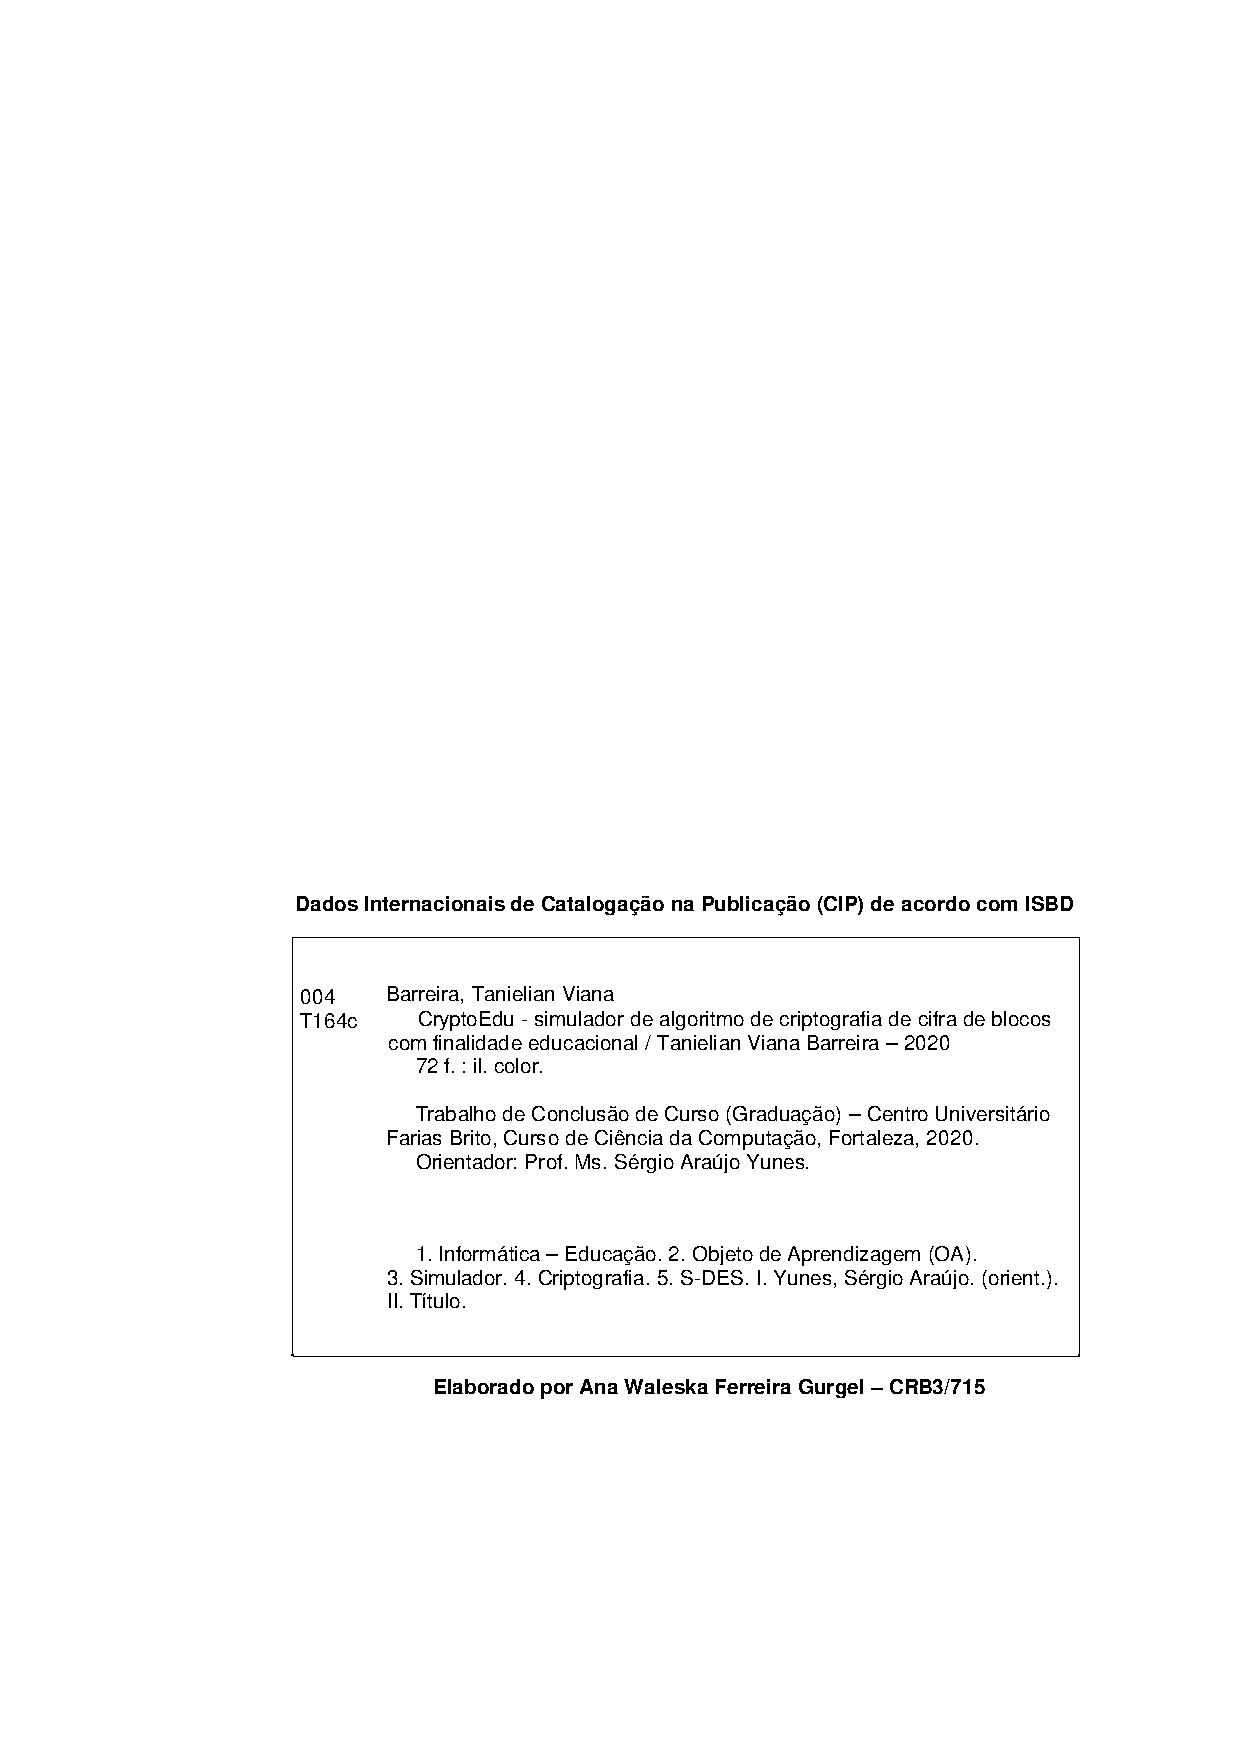
\includepdf{catalografica.pdf}
% Comando para colocar a folha de aceite do trabalho
%\includepdf{aceite.pdf}
%Remove página branca extra entre capítulos
\cleardoublepage

% Dedicatória
\begin{dedicatoria}
   \vspace*{\fill}
   \centering
   \noindent
   \textit{
    Dedico este trabalho a todos os que me ajudaram ao longo desta caminhada. Especialmente aos meus pais, amigos e esposa.
   }
   \vspace*{\fill}
\end{dedicatoria}

% Agradecimentos
\begin{agradecimentos}
    Agradeço ao professor Dr. Jorge Albuquerque por ter me apresentado à Computação, esta área que tanto amo.
    
    Agradeço aos professores Dr. Fani Carvalho, Cleiton Albuquerque, Ricardo, Maikol.
    
    E agradeço especialmente ao meu orientador Me. Sérgio Araújo Yunes por ter me auxiliado na criação deste trabalho, mas principalmente, pela paciência.
    
    \revisar{Melhorar...}
\end{agradecimentos}

% Resumos
%\setlength{\absparsep}{18pt} % ajusta o espaçamento dos parágrafos do resumo
\begin{resumo}
    A manipulação de informações sensíveis, senhas, dinheiro e informações privadas, por meio da \textit{internet} faz com que a segurança da informação seja um ponto que, cada vez, mais deve ser levado em consideração ao se manipular dados, seja ao persistir ou ao trafegar estes. A criptografia, um dos pilares da segurança da informação, por sua vez, é complexa, dificultando assim o seu ensino e, consequentemente, sua utilização de maneira adequada ou otimizada. Vale a pena salientar também, que o uso de \acrfull{oas} para melhorar o processo de ensino-aprendizagem vem crescendo cada vez mais e as suas áreas de aplicabilidade também. Isso é decorrente dos vários benefícios provenientes da utilização de \acrshort{oas} no ambiente de ensino, em especial no \acrfull{ead}. Baseado no contexto exposto, este trabalho apresenta o resultado de uma pesquisa na área da Informática na Educação, que objetivou criar um \acrlong{oa} simulador capaz de auxiliar no processo de ensino-aprendizagem de algoritmos criptográficos por cifra de bloco. No simulador, são explicadas todas as etapas do algoritmo simulado que, por ser o mais adequado ao ensino, é o S-DES. Além disso, foi realizada uma pesquisa com intuito de avaliar a efetividade do \acrshort{oa} no processo de ensino-aprendizagem e esta atestou que o simulador foi capaz de aumentar o conhecimento de alunos e professores sobre a temática abordada.
    
    \vspace{\onelineskip}
    \noindent 
    \textbf{Palavras-chave}:  Informática na Educação, \acrfull{oa}, Simulador, Criptografia, S-DES
\end{resumo}
\cleardoublepage
\begin{resumo}[Abstract]
    \begin{otherlanguage*}{english}
    The manipulation of sensitive information, passwords, money, and private information, through the internet, makes information security a point that more and more, must be taken into account when manipulating data, either when persisting or when trafficking these. Cryptography, one of the pillars of information security, in turn, is complex, making it difficult to teach and, consequently, to use in an appropriate or optimized way. It is also worth noting that the use of Learning Objects (LOs) to improve the teaching-learning process has been growing more and more and its areas of applicability as well. This is due to the various benefits arising from the use of LOs in the teaching environment, especially in Distance Learning (DL). Based on the given context, this work presents the result of a research in the field of Computers in Education, which aimed to create a simulator capable of assisting in the teaching-learning process of block cipher cryptographic algorithms. In the simulator, all stages of the simulated algorithm S-DES are explained, the reason for that being the fact that this is the most suitable algorithm for teaching. In addition to that, a survey was carried out in order to assess the effectiveness of the LO in the teaching-learning process and this asserted that the simulator was able to increase the knowledge of students and teachers on the addressed topic.
    
    \vspace{\onelineskip}
    \noindent 
    \textbf{Keywords}: Computers in Education, Learning Object, Simulator, Cryptography, S-DES
    \end{otherlanguage*}
\end{resumo}

\begin{epigrafe}
    \vspace*{\fill}
	\begin{flushright}
		\textit{
		    "Antes tarde do que nunca"
		}
	\end{flushright}
\end{epigrafe}

%Lista de Siglas
\printglossary [type=\acronymtype, title=Lista de Siglas e Abreviações, toctitle=Lista de Siglas e Abreviações]
\cleardoublepage

% inserir lista de ilustrações
\pdfbookmark[0]{\listfigurename}{lof}
\listoffigures*
\cleardoublepage

% inserir o sumario
\pdfbookmark[0]{\contentsname}{toc}
\tableofcontents*
\cleardoublepage

% ----------------------------------------------------------
% ELEMENTOS TEXTUAIS
% ----------------------------------------------------------
\textual

%inclui novas arquivos .tex ao trabalho na ordem em que são incluidos aqui
\chapter{Introdução}
\label{char:intro}
Várias aplicações da Ciência da Computação possuem como necessidade o conhecimento de como funcionam os métodos e técnicas da Criptografia. Essa necessidade decorre do fato de que a \textit{Internet} (principalmente utilizada em dispositivos móveis), definitivamente, está inserida na vida cotidiana das pessoas e novos costumes estão sendo adotados pela sociedade. O comércio eletrônico, as operações bancárias de transferência eletrônica de fundos, o uso do cartão de crédito como moeda de plástico, por exemplo, se constituem na realidade do convívio social, independente de qual seja a sua posição social. Tornando a segurança da informação um ponto cada vez mais importante ao se manipular/trafegar dados.\cite{silva09} \cite{silva12}

A alta complexidade dos algorítimos usados nas aplicações da Criptografia faz com quê o processo de ensino-aprendizagem destes nem sempre seja eficiente, principalmente se os algoritmos forem ensinados e analisados na sua complexidade total \cite{silva09} \cite{silva12}. A academia apresenta aos profissionais em formação na área de Ciência da Computação representações simplificadas do mundo real, embora ainda próximas do mundo real (quanto mais próximas, melhor), com o intuito de facilitar o manuseio dessa representação no ambiente de estudo \cite{maia01} \cite{maia03} \cite{kioki08}. Naturalmente, a abordagem de cunho pedagógico precisa preservar os aspectos fundamentais da arquitetura de cada algoritmo \cite{garmpis11} \cite{lopes12}.

Analisando o contexto acima apresentado, Esse trabalho apresenta uma ferramenta capaz de auxiliar no processo de ensino-aprendizagem de algorítimos criptográficos por cifra de bloco nas disciplinas que abordem a criptografia. A ferramenta possibilita a simulação da execução da versão simplificada do algoritmo criptográfico de chave simétrica conhecido como \acrfull{des}. Esse simulador permite que o algorítimo seja executado passo a passo, tanto de maneira sequencial como cada passo, até mesmo cada etapa dentro de um passo, isoladamente. Cada etapa possui sua explicação e execução bit a bit. Esta é apresentada no capítulo \ref{char:ferrdesenvolvida}.

Além disso, foi realizada uma pesquisa de campo com intuito de avaliar a efetividade da ferramenta no processo de ensino-aprendizagem. Os resultados dessa pesquisa são apresentados no capítulo \ref{char:pesquisa}.

\chapter{Fundamentação Teórica}
\label{char:fundteorica}
Inicia-se com uma explicação geral sobre o enquadramento desse trabalho no meio acadêmico com os tópicos \ref{sec:informaticaeducacao} \nameref{sec:informaticaeducacao} e \ref{sec:objetosaprendizagem} \nameref{sec:objetosaprendizagem}.
 
No tópico \ref{sec:ferramentaspoioensino} \nameref{sec:ferramentaspoioensino}, é dado uma visão geral sobre o que são e sobre o ganho que elas trazem para os alunos. O tópico, \ref{sec:simuladoresvoltadosensino} \nameref{sec:simuladoresvoltadosensino}, traz uma visão geral sobre simuladores e uma análise da existência de simuladores voltados ao ensino de uma forma geral e o tópico \ref{sec:simuladorescriptografia} enumera os simuladores de criptografia atuais.

A análise criptográfica inicia-se com o tópico \ref{sec:historia} \nameref{sec:historia}, onde há uma breve contextualização histórica sobre segurança e criptografia. No tópico \ref{sec:criptografia} \nameref{sec:criptografia}, é feita uma visão geral sobre criptografia e suas aplicabilidades. 

Os dois seguintes, \ref{subsec:criptografiasync} \nameref{subsec:criptografiasync} e \ref{subsec:criptografiaasync} \nameref{subsec:criptografiaasync}, tratam de dois tipos de criptografia e explanam sobre suas definições, seus cenários de utilização, e trazem alguns exemplos de algoritmos sobre seus respectivos ramos da criptografia. O tópico \ref{sec:cifradeblocos} \nameref{sec:cifradeblocos} fala sobre esse método de criptografia simétrica no qual é feita uma visão geral sobre seu funcionamento e benefícios obtidos por sua utilização.

Os tópicos \ref{sec:des} \nameref{sec:des}, \ref{sec:3des} \nameref{sec:3des} e \ref{sec:sdes} \nameref{sec:sdes} tratam sobre estes algoritmos de criptografia simétrica baseados em cifra de blocos, os quais trazem uma visão geral e uma breve explicação de cada algoritmo dando uma ênfase maior no \nameref{sec:sdes} por ser o algorítimo utilizado na ferramenta desenvolvida.

Neste caso, é perceptível a intenção de trazer uma clara e breve explanação sobre os tópicos abordados neste trabalho, de forma que este se faça compreender da melhor forma possível.

\section{Informática na educação}
\label{sec:informaticaeducacao}
A educação abrange dar e receber conhecimento. Qualquer sociedade possui esse cenário, que é responsável pela manutenção e propagação às gerações que se seguem, da cultura necessária à convivência de um membro na sua sociedade \cite{hamawaki09}.

Dentre as formas de aprendizagem, são citadas duas teorias importantes por Ausubel \cite{ausubel80}, a aprendizagem significativa e a mecânica.

A primeira diz respeito à ideia de que a aprendizagem é um processo por onde uma informação recém-adquirida relaciona-se com um aspecto importante da estrutura de conhecimento do aluno, ou seja, quando a nova informação adquirida vincula-se em conhecimentos relevantes previamente adquiridos na estrutura cognitiva do aluno. A aprendizagem significativa é onde o aluno realmente aprende.

A aprendizagem mecânica por sua vez ocorre quando o novo conhecimento se associa pouco ou não se associa a algum conhecimento importante já existente na estrutura cognitiva do aprendiz. Quando isso ocorre o conhecimento adquirido recentemente é gravado de maneira arbitrária. Essa aprendizagem é inviável quando um aluno recebe um novo conhecimento em uma área de conhecimentos nova para ele. Ou seja, aprendizagem mecânica acontece somente até que alguns elementos do conhecimento pré-adquirido, relevantes a novas informações na mesma área de conhecimento, existam na estrutura cognitiva do aluno e possam ser utilizadas como base para a aprendizagem significativa. E é através dessa aprendizagem que se inicia a criação, na cabeça do aluno, de uma estrutura cognitiva mais complexa, onde ele deixa de aprender de forma passiva e mecânica e passa a assimilar o conteúdo de forma mais clara e não linear \cite{ausubel80}.

Muitas vezes o desempenho da transmissão do conhecimento é árduo e complexo. Tendo em vista essa dificuldade, almeja-se a utilização bons recursos didáticos que melhorem o desempenho docente. \cite{souza07}.

Uma das considerações que devem ser levadas em conta pelo educador como critério de escolha de um recurso didático é que sua utilização deve preencher as lacunas existentes no ensino tradicional e viabilizar ao aluno a ampliação 
tanto da capacidade de reter conhecimento quanto a sua visão, e ainda estimular o ensino docente. \cite{trivelato06}

Sons, imagens, construção de maquetes e até o uso de materiais lúdicos, esses simples elementos podem ser aplicados como recursos didáticos. Quando o corpo docente se utiliza de tipos variados de recursos didáticos ele não somente faz com que o ensino seja mais interessante do que o ensino tradicional, como também pode propiciar melhores resultados \cite{parra85} \cite{souza07} \cite{costoldi09}. Dentre os recursos didáticos que podem ser utilizados existem vários tipos, como: livros, apostilas, artigos, quadro e giz, apresentações, maquetes, trabalhos acadêmicos, softwares, ilustrações, filmes, músicas, exercícios físicos, excursões, brincadeiras e outros \cite{ferreira07}. A brincadeira Adedonha, por exemplo, já teve sua eficiência comprovada como ferramenta prático-pedagógica no processo de ensino-aprendizagem \cite{silva18}.

A abordagem do uso do computador e/ou dispositivos eletrônicos similares como recurso pedagógico utilizado pelo docente no processo de ensino do corpo discente é conhecido como Informática na educação. \cite{kenski07}

\section{Objetos de aprendizagem}
\label{sec:objetosaprendizagem}

\textit{"...definimos objetos de aprendizagem como sendo recursos digitais dinâmicos, interativos e reutilizáveis em diferentes ambientes de aprendizagem elaborados a partir de uma base tecnológica. Desenvolvidos com fins educacionais, eles cobrem diversas modalidades de ensino: presencial, híbrida ou à distância; diversos campos de atuação: educação formal, corporativa ou informal; e, devem reunir várias características como durabilidade, facilidade para atualização, flexibilidade, interoperabilidade, modularidade, portabilidade, entre outras. Eles ainda apresentam-se como unidades autoconsistentes de pequena extensão e fácil manipulação, passíveis de combinação (essa combinação dá-se, principalmente, no sentido objeto-mídia, mas o contrário também é válido dependendo da mídia, pois não são todas que oferecem a característica de hiperligação) com outros objetos educacionais ou qualquer outra mídia digital (vídeos, imagens, áudios, textos, gráficos, tabelas, tutoriais, aplicações, mapas, jogos educacionais, animações, infográficos, páginas web) por meio da hiperligação. Além disso, um objeto de aprendizagem pode ter usos variados, seu conteúdo pode ser alterado ou reagregado, e ainda ter sua interface e seu layout modificado para ser adaptado a outros módulos ou cursos. No âmbito técnico, eles são estruturas autocontidas em sua grande maioria, mas também contidas, e marcadas por identificadores denominados metadados."} \cite{audino12}

Em suma, um \acrfull{oa} é um recurso digital utilizado para suportar o ensino. Imagens, vídeos, softwares e animações podem ser considerados \acrshort{oa}s contanto que sejam voltados ao ensino. Já os \acrshort{avas} por sua vez, \acrlong{avas}, não são considerados \acrshort{oa}s pois esses, apesar de gerenciar e até armazenar \acrshort{oa}s, não são utilizados diretamente na aprendizagem. \cite{wiley02} \cite{braga14}

Apesar do AVA ser o principal instrumento mediador em um sistema de \acrfull{ead} isso não exclui sua utilização como suporte para o ensino presencial \cite{belmonte10}.

\section{Ferramentas de apoio ao ensino}
\label{sec:ferramentaspoioensino}

Ainda é um desafio a criação de \acrshort{oa}s pois geralmente o conhecimento pedagógico é detido por um profissional da área de ensino e este normalmente não possui o conhecimento técnico avançando necessário para o desenvolvimento de \acrshort{oa}s \cite{braga15}.

Há também \acrshort{oa}s que podem ser customizadas e aplicadas para várias áreas de ensino, como é o caso do jogo \textit{Minecraft: Education Edition} que já foi aplicado no ensino de Biologia, Ecologia, Física, Química, Geologia, Geografia \cite{short12} e até Cibersegurança \cite{geary19}, .

Existe um problema comum entre professores e alunos de disciplinas do curso de Ciência da Computação, e este é: Existe uma dificuldade em demonstrar a real dinâmica dos eventos computacionais. Por melhor que o mestre possua conhecimento e comunicação, que o aluno dedique raciocínio e atenção, a total compreensão dos conceitos abordados fica comprometida pela forma de abordagem das disciplinas.

O computador não deve ser o substituto do professor, mas sim, tomar o papel de ferramenta educacional auxiliando o aprendizado. Com isso o papel do professor passa a ser mais produtivo.

Primeiramente, ferramentas voltadas ao ensino, já se utilizando do computador, se baseavam na máquina de \textit{B. F. Skinner}, onde se utilizava a ideia de instrução programada, que consistia de dividir o conteúdo total em pequenas partes lógicas e sequenciais.

Somente durante a década de 1960, foi dado inicio ao conceito de \acrfull{cai}, ou seja, \acrfull{pec}. A real dispersão do \acrshort{cai} só aconteceu com popularização dos microcomputadores, possibilitando assim, a criação de diversos tipos de ferramentas de ensino, como, tutoriais, exercício-e-prática, avaliações, jogos, e simulações \cite{hamawaki09}.

\section{Simuladores voltados ao ensino}
\label{sec:simuladoresvoltadosensino}

Algumas situações são tão singulares, que se preparar para tais torna-se difícil. E portanto, com o intuito de proporcionar a alguém um conhecimento maior sobre estas situações os simuladores foram criados.

A simulação é uma representação do mundo real. As primeiras simulações foram criadas com o intuito de disponibilizar um ambiente seguro para situações que envolvessem risco ao humano. Dentre elas podemos citar simulações de viagens e mergulhos profundos. Posteriormente, foram criadas com o intuito de se obter uma economia, seja ela de tempo e/ou dinheiro, que é o caso da indústria automobilística e aviação.

Diversas são as áreas de conhecimento que fazem uso das simulações \cite{banks09}. Na ciência da computação há uma disponibilidade de simuladores, cada um atendendo a uma respectiva disciplina, assim como redes de computadores, arquitetura de computadores, técnicas de programação e sistemas operacionais.

Os simuladores possuem um potencial bem maior do que as outras ferramentas de ensino citadas acima. A aplicação de simulações no universo acadêmico permite que o aluno desenvolva hipóteses, teste-as, analise os resultados e concretize seus conhecimentos. Simuladores devem ser utilizados como ferramenta complementar as aulas lecionadas pelo professor.

Mesmo com todas as vantagens envolvidas, o desenvolvimento de um simulador não é algo trivial. Uma vez que a ferramenta possui um cunho pedagógico, a utilização de recursos multimídia para tornar a simulação mais fiel à realidade é muito importante, e a utilização destes recursos não é algo de simples desenvolvimento.

Quando o aluno possui pouco conhecimento na área, os simuladores são indicados como melhor ferramenta de auxilio. Principalmente, se forem para auxiliar cursos de extensão e graduação \cite{maia01} \cite{maia03}. 

\section{Simuladores de criptografia}
\label{sec:simuladorescriptografia}

\subsection{CyberChef}
Um simulador da máquina enigma criado pela \acrfull{gchq}, o centro de inteligência britânica.

\begin{figure}[H]
    \centering
    \caption{Simulador: CyberChef}
    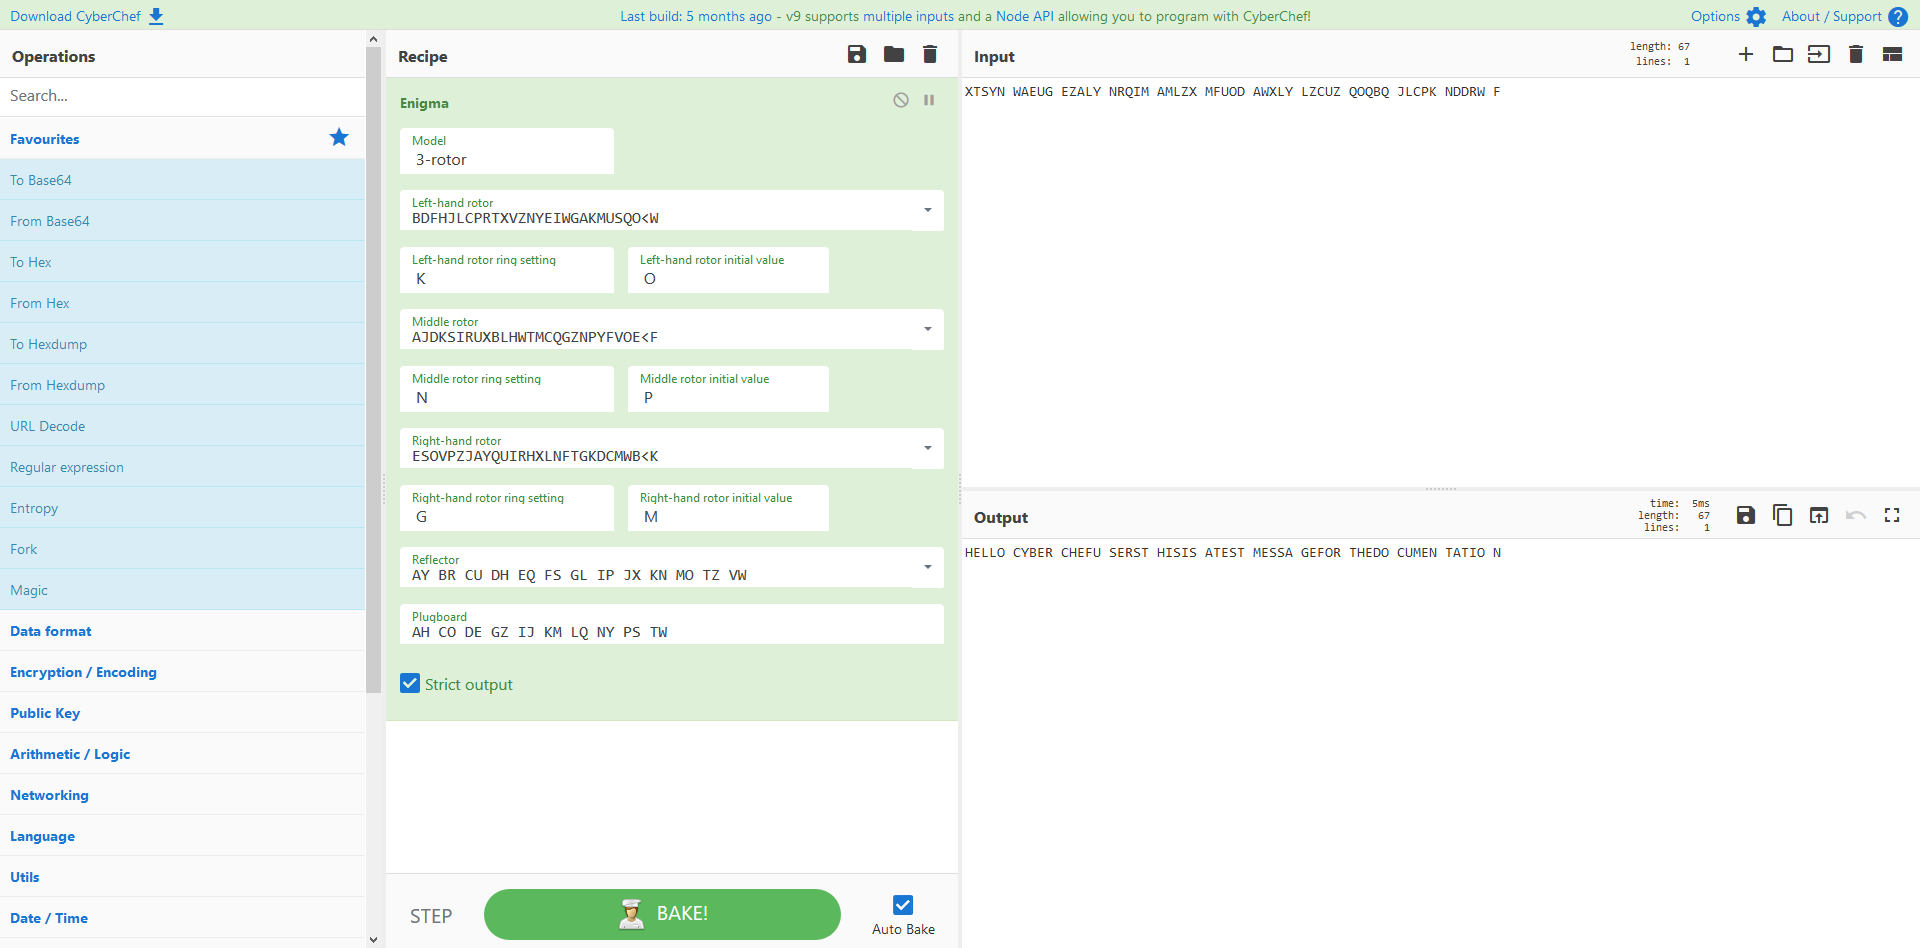
\includegraphics[width=1\linewidth]{Simuladores/CyberChef_Enigma.png}
    \legend{Fonte: \textit{https://gchq.github.io/CyberChef/}}
\end{figure}

Principais características:
\begin{itemize}
    \item Disponibilizado \textit{online} em \textit{https://gchq.github.io/CyberChef/}.
    \item Idioma: Inglês.
    \item Possui vários algorítimos simples.
    \item Mostra somente entradas e saídas.
    \item Possui atualmente vários algorítimos.
    \item Pode encadear criptografias que serão aplicadas sequencialmente sobre o \textit{input}.
    \item Não é direcionado ao ensino.
    \item Disponibilizado no \textit{GitHub} (\textit{https://github.com/gchq/CyberChef/}).
\end{itemize}

\subsection{CrypTool}

\textit{CrypTool} é um portal de criptografia (\textit{https://www.cryptool.org/en/}) que disponibiliza alguns simuladores de criptografia.

\subsubsection{CrypTool 2}

\begin{figure}[H]
    \centering
    \caption{Simulador: CrypTool 2}
    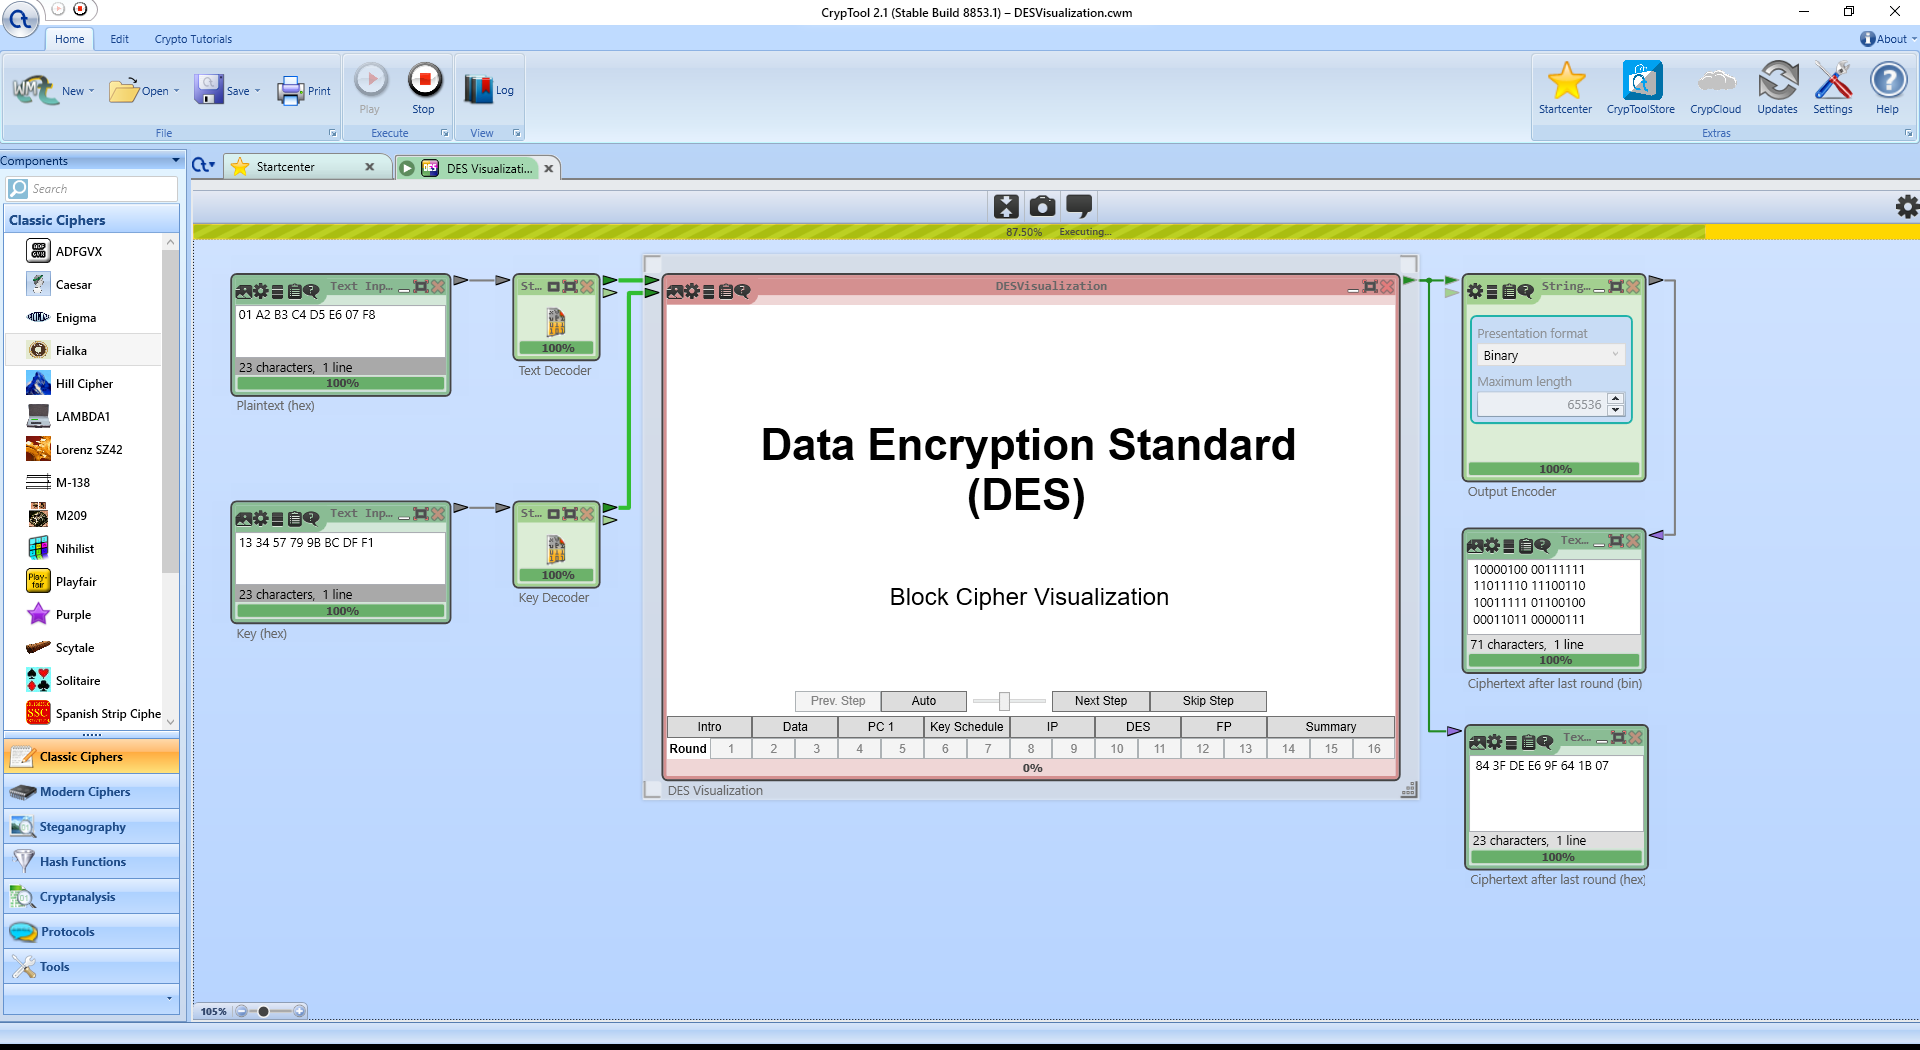
\includegraphics[width=1\linewidth]{Simuladores/CrypTool2.png}
\end{figure}

Principais características:
\begin{itemize}
    \item Só pode ser instalado em Windows.
    \item Idioma: Inglês.
    \item Tem um conjunto de \textit{templates} de algorítimos expansível.
    \item Possui somente 1 \textit{template} que executa passo a passo.
    \item Interface complexa e de difícil utilização.
    \item Não é direcionado ao ensino.
\end{itemize}

\subsubsection{JCrypTool}

\begin{figure}[H]
    \centering
    \caption{Simulador: JCrypTool}
    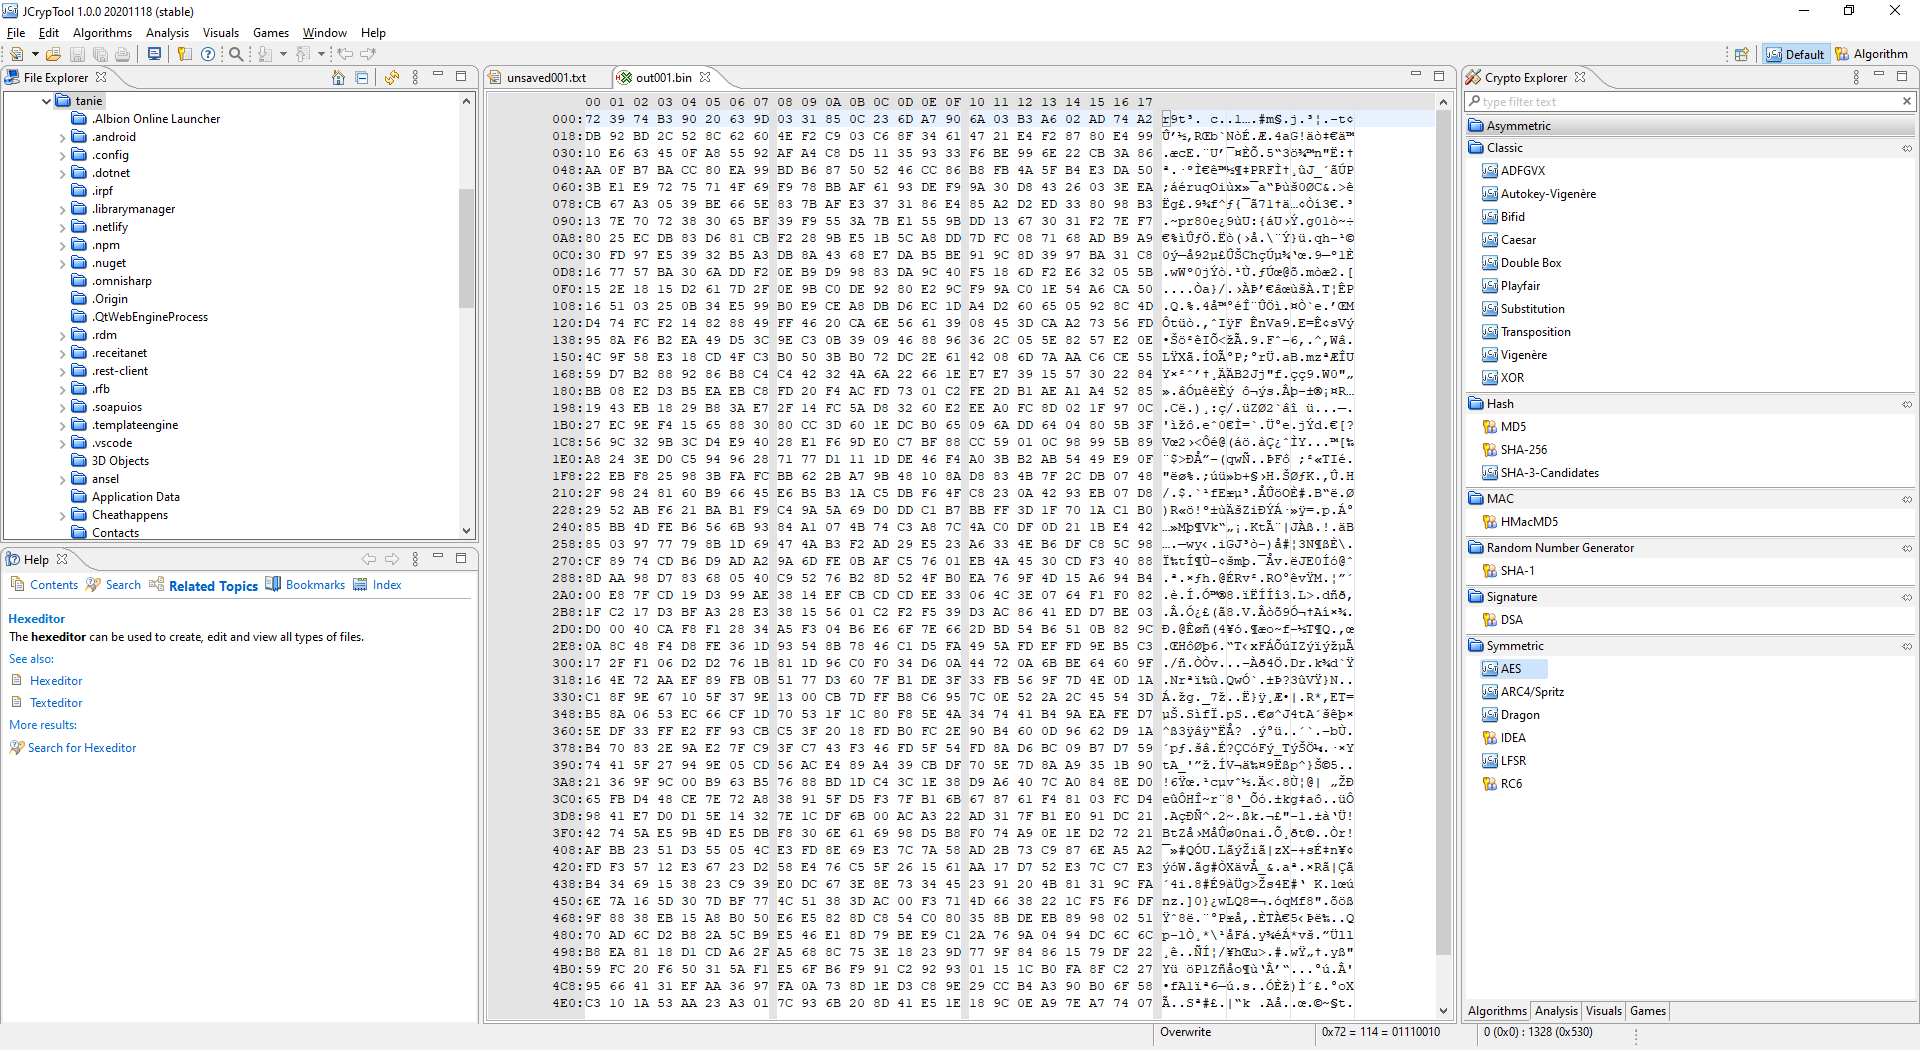
\includegraphics[width=1\linewidth]{Simuladores/JCrypTool.png}
\end{figure}

Principais características:
\begin{itemize}
    \item Desenvolvida em Java e pode ser instalado em Linux, Mac and Windows.
    \item Idioma: Inglês.
    \item Tem um conjunto de \textit{templates} de algorítimos expansível.
    \item Não possui \textit{template} que executa passo a passo.
    \item Interface complexa e de difícil utilização.
    \item Não é direcionado ao ensino.
\end{itemize}

\subsection{S-DES Simulator (\textit{Android App})}

\begin{figure}[H]
    \centering
    \caption{Simulador: S-DES Simulator}
    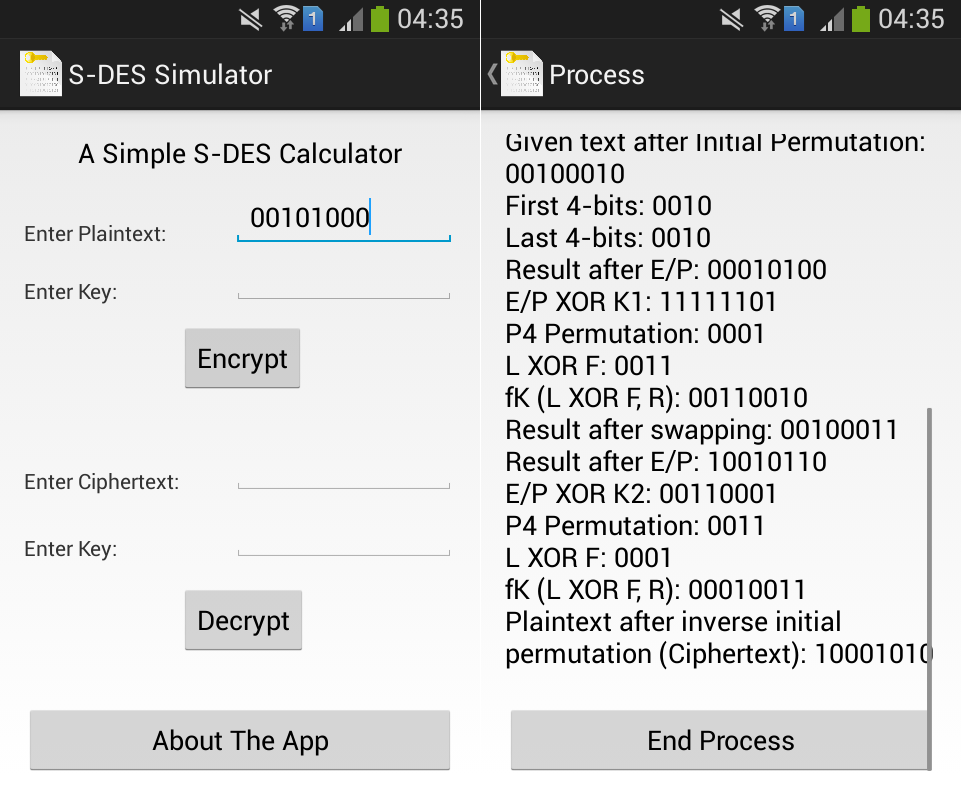
\includegraphics[width=.75\linewidth]{Simuladores/SDESSimulatorApp.png}
\end{figure}

Principais características:
\begin{itemize}
    \item Pode ser instalado em versões antigas do \textit{Android}. Foi necessário usar um simulador para poder testar.
    \item Idioma: Inglês.
    \item Só possui o \acrshort{sdes} como possível algorítimo.
    \item Executa passo a passo mas só mostra os resultados dos passos.
    \item É direcionado ao ensino.
\end{itemize}

\subsection{S-DES Simulator (Koreano)}

\begin{figure}[H]
    \centering
    \caption{Simulador: S-DES Simulator}
    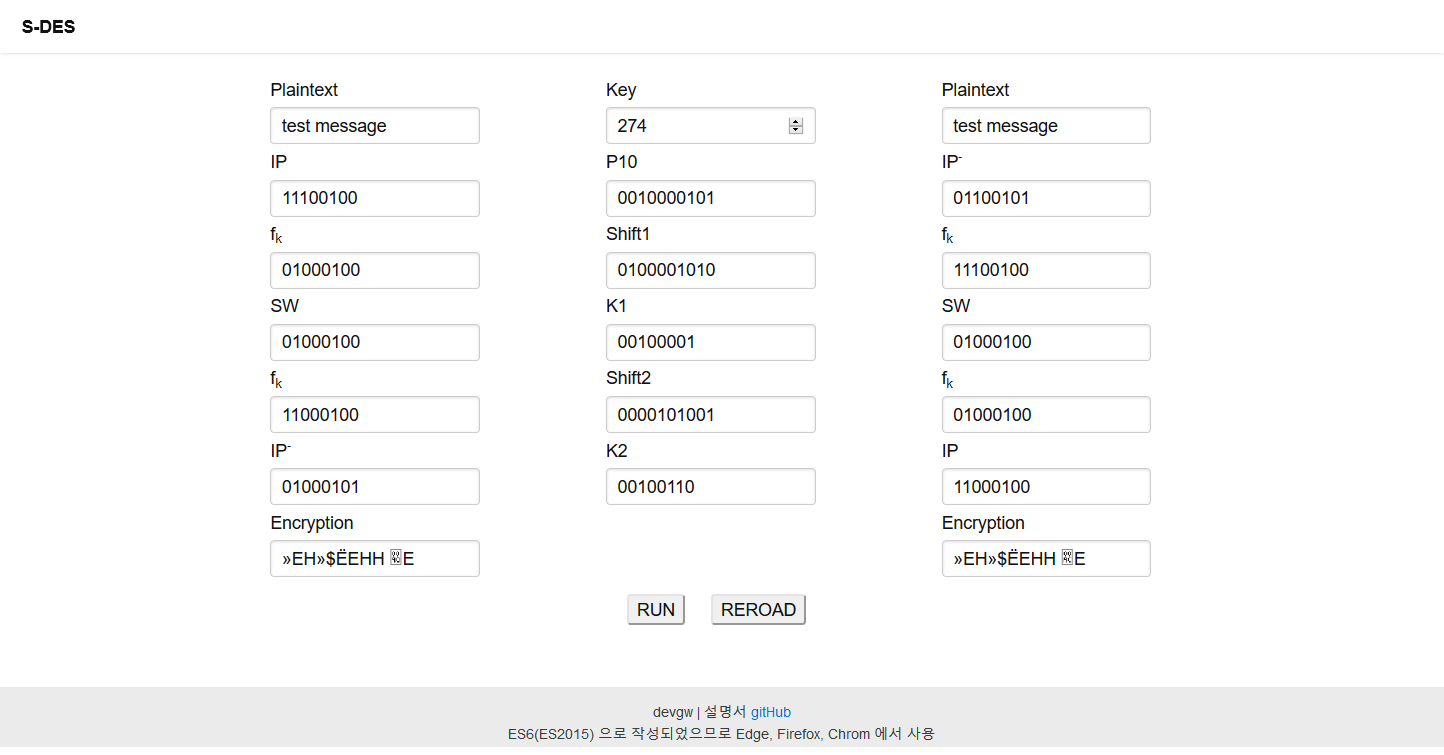
\includegraphics[width=.75\linewidth]{Simuladores/SDESSimulatorKr.png}
\end{figure}

Principais características:
\begin{itemize}
    \item Disponibilizado \textit{online} em \textit{https://devgw.github.io/S-DES-simulator/}.
    \item Idioma: Koreano.
    \item Só possui o \acrshort{sdes} como possível algorítimo.
    \item Executa passo a passo mas só mostra os resultados dos passos.
    \item É direcionado ao ensino.
    \item Disponibilizado no \textit{GitHub} (\textit{https://github.com/devGW/S-DES-simulator}).
\end{itemize}

\subsection{S-DES Simulator (Inglês)}

\begin{figure}[H]
    \centering
    \caption{Simulador: S-DES Simulator}
    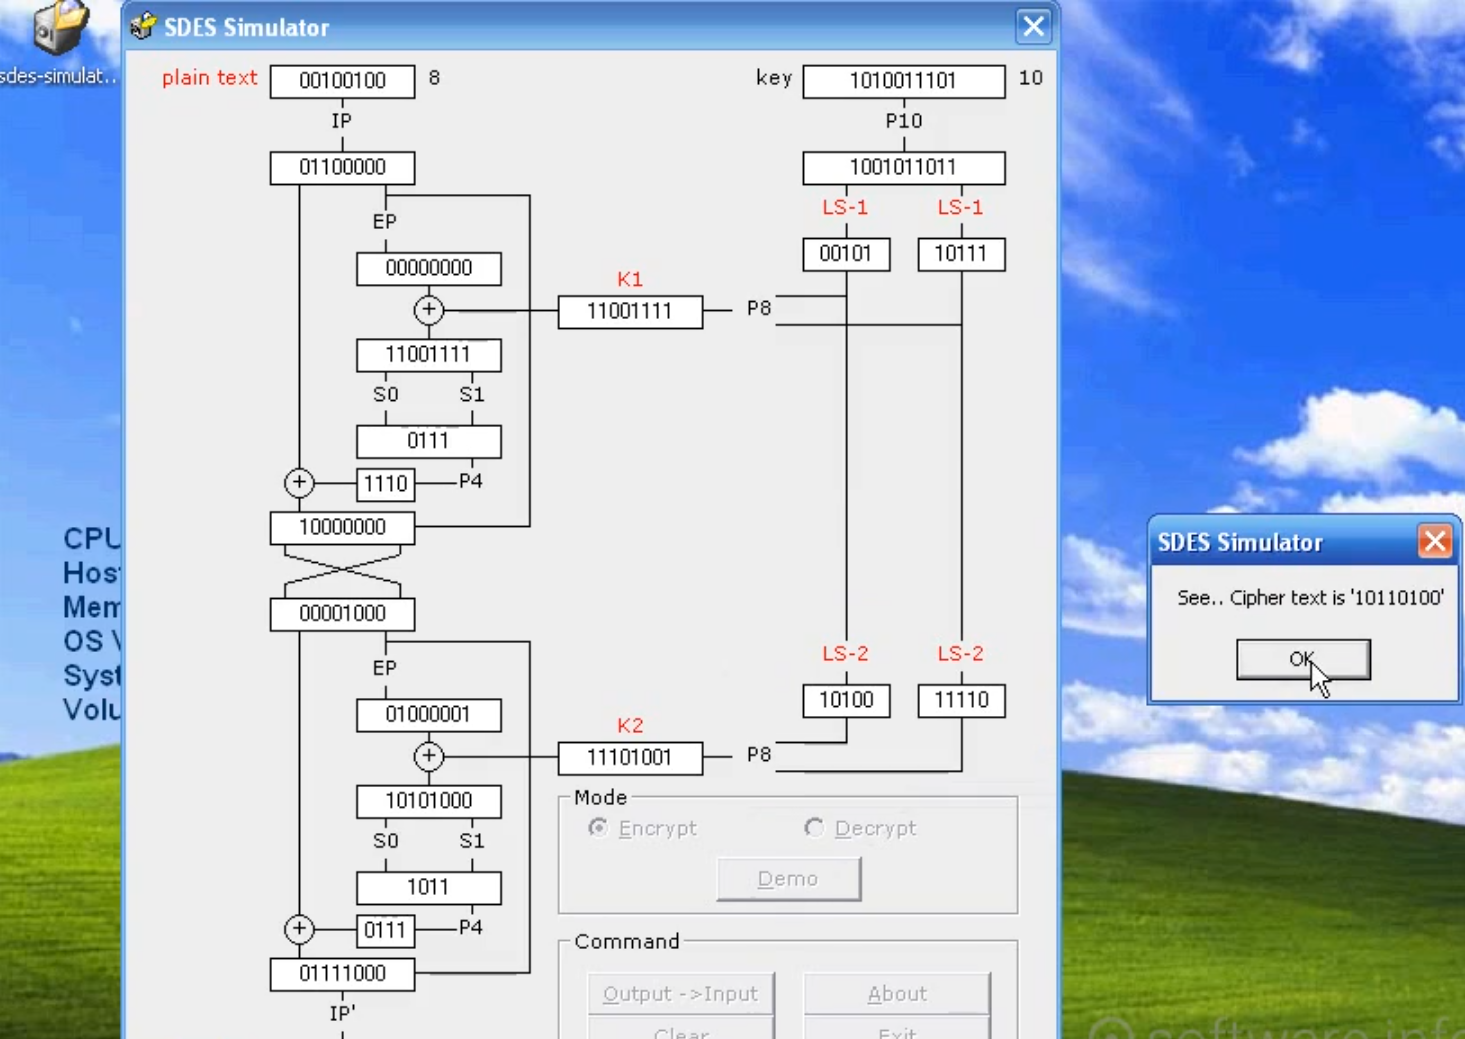
\includegraphics[width=.75\linewidth]{Simuladores/SDESSimulatorXp.png}
\end{figure}

Principais características:
\begin{itemize}
    \item Só pode ser instalado em Windows.
    \item Idioma: Inglês.
    \item Só possui o \acrshort{sdes} como possível algorítimo.
    \item Executa passo a passo mas só mostra os resultados dos passos.
    \item É direcionado ao ensino.
\end{itemize}

\subsection{Crypto-tutor}
\textit{"Crypto-tutor: An educational tool for learning modern cryptography"} \cite{luburic16} possui como principais características:
\begin{itemize}
    \item Idioma: Inglês.
    \item Possui vários algorítimos.
    \item Possui \textit{benchmarking} entre os algorítimos.
    \item É direcionado ao ensino.
\end{itemize}

\subsection{CET - \textit{Cryptographic Education Tool}}
CET - \textit{Cryptographic Education Tool} \cite{abuzaid11} possui como principais características:
\begin{itemize}
    \item Idioma: Inglês.
    \item Possui os algorítimos \textit{simple cipher}, \acrshort{rsa} e \acrshort{sdes}.
    \item É direcionado ao ensino.
\end{itemize}

\section{História}
\label{sec:historia}
Há algumas décadas atrás, antes que se fosse comum o uso de equipamentos de processamento de dados, a segurança da informação que era considerada importante para uma empresa se dava basicamente através de dois meios: o administrativo e o físico. Um bom exemplo para o meio administrativo é o uso de um processo de aquisição de profissionais bastante seleto e rigoroso, assim como a utilização de um contrato de confidencialidade que protege a empresa de possíveis ‘vazamentos’ de dados. Um bom exemplo para o meio físico é o uso de cofres e senhas para armazenar documentos importantes ou até confidenciais.

Com o surgimento do computador surgiu a necessidade de proteger virtualmente os arquivos, agora armazenados de forma virtual no computador. Essa necessidade é ainda mais evidente com o surgimento da Internet, que traz uma facilidade de comunicação muito grande entre os computadores.

O \acrfull{iab} emitiu, em 1994, um relatório de título “Security in the internet architecture” (Segurança na arquitetura da Internet). O documento estabelecia que a internet necessitava de mais e melhor segurança. Entre as principais áreas citadas no relatório como sendo as que mais necessitavam de segurança estavam a infraestrutura da rede contra monitoração e controle não autorizados do tráfego da rede e também a necessidade de proteger o tráfego entre usuários finais se utilizando de autenticações e criptografias.

Com o passar dos anos, os ataques através da Internet se tornaram mais evoluídos, eles se tornaram mais automatizados e mais devastadores, necessitando cada vez mais de formas de segurança também mais evoluídas \cite{stallings14}.

Existe uma lista de mecanismos de segurança explicitados na recomendação X.800 \cite{itu91}. Entre eles temos a cifragem, que é melhor descrita mais adiante. A X.800 divide, muito claramente, dois tipos de criptografia, a reversível e a irreversível. A criptografia reversível é composta por um algoritmo matemático que permite que dados sejam criptografados e que estes dados criptografados possam ser decriptografados posteriormente. Já a criptografia irreversível, por sua vez, é capaz de criptografar os dados, mas a decriptografia desses dados é impossível. Esta por sua vez tem objetivos diferentes da reversível, que visa somente trafegar ou armazenar dados de maneira segura, ela é composta de algoritmos de hash e tem como objetivo autenticação e assinatura digital \cite{stallings14} \cite{itu91}.

\section{Criptografia}
\label{sec:criptografia}
Segundo a National Research Council (1991, apud STALLINGS, 2008, pg. 15), “A criptografia provavelmente é o aspecto mais importante da segurança de comunicações e está se tornando cada vez mais importante como um componente básico para a segurança do computador.”.

O termo Criptografia vem do Grego \textit{kryptós}, que significa “escondido” e de \textit{gráphein}, que significa “escrita”. Ela é o estudo dos princípios e técnicas pelas quais os dados podem ser transformados da sua forma original em outra ilegível. Dessa forma, os dados podem ser conhecidos somente pelo destinatário, o detentor da “chave secreta”, o que faz com que mesmo que tenham sido interceptados, torne difícil a leitura de seu conteúdo por alguém não autorizado. Ela faz parte da Criptologia e é um sub-ramo da Matemática \cite{knudsen98}.

O estudo da maneira de camuflar o real significado de uma mensagem usando técnicas e algoritmos de cifragem têm evoluído juntamente com o estudo da maneira de se conseguir entender a mensagem quando não se é o real destinatário da mesma. Este campo de estudo é chamado Criptoanálise \cite{gaines56}. A Criptologia engloba a Criptografia e a Criptoanálise. Alguns autores se utilizam do termo Criptovirologia quando falam de vírus que se utilizam de chaves publicas \cite{young04}.

Há também a Esteganografia que não faz parte de Criptologia, mesmo sendo estudada em situações bem similares e até pelos mesmos autores. Ao contrário da criptografia que modifica a informação com intuito de transformar seu estado original em algo indecifrável a Esteganografia estuda formas de como se pode camuflar uma informação dentro de outra. Temos também a Esteganálise que está para Esteganografia assim como a Criptoanálise está para a Criptografia \cite{salomon05}.

A criptografia se divide em Simétrica, também chamada de criptografia convencional, e Assimétrica, também chamada de criptografia por chave pública \cite{stallings14} e dentro dessa divisão ainda temos algoritmos de criptografia reversíveis e irreversíveis \cite{stallings14} \cite{itu91}.

A criptografia possui inúmeras áreas de aplicação. Desde transações bancárias, envio de e-mails, segurança de arquivos sigilosos, segurança de autenticação, armazenamento de senhas em bancos de dados até o sinal de linha telefônica, sinal de TV digital e acesso a sites certificados \cite{avelino07}.

\subsection{Criptografia Simétrica}
\label{subsec:criptografiasync}
Também chamada de criptografia convencional, a criptografia simétrica é um criptosistema onde tanto a criptografia como a decriptografia são realizadas com a mesma chave.

Ela transforma uma mensagem clara em uma mensagem cifrada, usando um algoritmo de criptografia e uma chave. Esta mesma chave juntamente com a inversão do algoritmo utilizado (gerando assim o algoritmo de decriptografia do algoritmo), são necessários para que se possa obter a mensagem clara novamente a partir da mensagem cifrada, assim como demonstra a Figura 1.

\begin{figure}[H]
    \centering
    \caption{Criptografia Simétrica}
    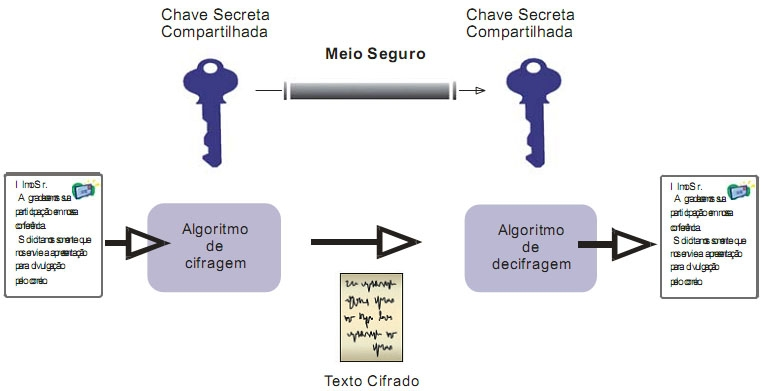
\includegraphics[width=.8\linewidth]{Figuras/CripSimetrica.jpg}
    \legend{Fonte: "Introdução à certificação digital: da criptografia ao carimbo de tempo" \cite{brocardo06}}
\end{figure}

Antes do computador, as cifras simétricas tradicionais poderiam se utilizar de técnicas de transposição ou de substituição, ou até as duas técnicas combinadas. Essas técnicas são os componentes básicos para todas as técnicas de criptografia.

Técnicas de transposição transpõem sistematicamente as posições dos elementos da mensagem clara. Tal técnica consiste na aplicação de alguma permutação na mensagem clara de forma que a mensagem final seja ilegível, e somente o detentor da forma de como os elementos da mensagem foram permutados pode obter novamente a mensagem de forma clara. A cifra mais simples dessa técnica é a cifra de \textit{Rail fence}. A Figura 2 ilustra como ficaria a crifa \textit{Rail fence} de profundidade dois do texto “Técnica de transposição”.

\begin{figure}[H]
    \centering
    \caption{Exemplo de \textit{Rail fence}}
    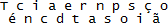
\includegraphics{Figuras/RailFence.png}
\end{figure}

Técnicas de substituição mapeiam elementos, caracteres ou bits, da mensagem clara e as substitui por outras letras ou números ou até símbolos. Analisando a mensagem clara como sendo um conjunto de bits, então a substituição é definida pela troca de padrões de bits da mensagem clara por padrões de bits da mensagem cifrada. Como exemplo clássico temos a cifra de César, criada por Júlio César. A Figura 3 ilustra como ficaria a cifra de César com o texto “Tecnica de substituicao”.

\begin{figure}[H]
    \centering
    \caption{Exemplo de cifra de César}
    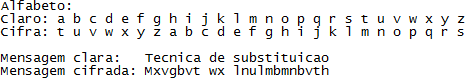
\includegraphics{Figuras/CifraDeCesar.png}
\end{figure}

Existem basicamente dois os ataques possíveis em um algoritmo criptográfico. A criptoanálise, que se baseia nas características do próprio algoritmo de criptografia, e a força bruta, que engloba simplesmente repetidas tentativas de todas as chaves possíveis até encontrar a correta.

Antes da existência do computador existiam máquinas que implementavam a nível de hardware técnicas de substituição. Eram conhecidas como máquinas de rotor. Duas foram as máquinas de rotor mais conhecidas, a da Alemanha, conhecida como Enigma e a do Japão conhecida como Purple. Elas foram utilizadas durante a segunda guerra mundial e a quebra desses dois códigos pelos Aliados foi significante para o resultado da guerra. Abaixo, a Figura 4 mostra a máquina Enigma com três rotores.

\begin{figure}[H]
    \centering
    \caption{Imagem da máquina Enigma}
    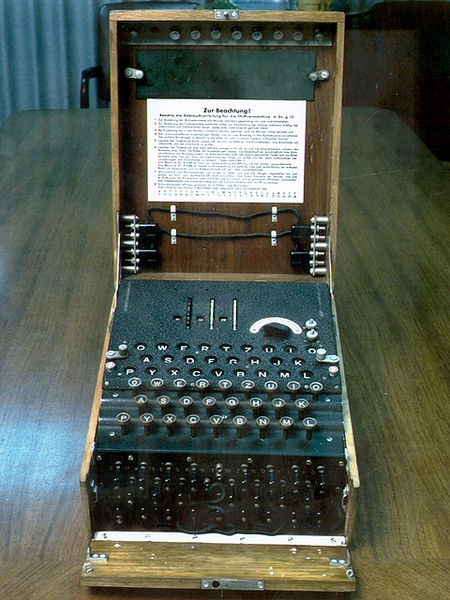
\includegraphics[width=.35\linewidth]{Figuras/MaqEnigma.jpg}
    \legend{Máquina Enigma com três rotores, teclado, luzes e conexões para câmbio de codificação. Fonte: Wikipedia \cite{maqenigma20}}
\end{figure}

Algoritmos simétricos são utilizados em cenários onde a mensagem tem uma necessidade de ser decriptografada, por exemplo, o Kerberos, serviço de autenticação desenvolvido no \textit{Massachusetts Institute of Technology} (MIT) como parte do projeto Athena, que visa trazer segurança a cenários distribuídos abertos, se utiliza unicamente de cifra simétrica \cite{stallings14}.

\subsection{Criptografia Assimétrica}
\label{subsec:criptografiaasync}
Também chamada de criptografia por chave pública, a criptografia assimétrica é um criptosistema onde a criptografia e a decriptografia são realizadas com chaves diferentes, uma pública e outra privada. Quando uma mensagem é criptografada com uma chave, somente a outra chave poderá decriptografar  a mensagem. O criptosistema assimétrico mais utilizado é o RSA.

Ela transforma uma mensagem clara em uma mensagem cifrada utilizando uma das duas chaves acima citadas e um algoritmo de criptografia. E utilizando a outra chave citada acima e o algoritmo de decriptografia, é possível extrair a mensagem clara a partir da mensagem cifrada.

A criptografia assimétrica possui três utilizações básicas: confidencialidade, autenticação ou ambas.

A confidencialidade garante que somente o destinatário será capaz de ler a mensagem. Quando se tem essa necessidade, deve-se criptografar a mensagem com a chave pública do destinatário, enviar a mensagem criptografada para o destinatário, e ele, de posse da chave privada, poderá decriptografar a mensagem e dessa forma obter a mensagem original.

O fato do destinatário ter conseguido decriptografar a mensagem com a chave privada dele próprio garante que a mensagem só poderia ter sido decriptografada por ele, detentor da chave privada, mas não garante a identidade do remetente, visto que a chave utilizada para criptografar a mensagem é publica, assim como demonstra a Figura 5.

\begin{figure}[H]
    \centering
    \caption{Fluxo da mensagem criptografada quando o foco é confidencialidade}
    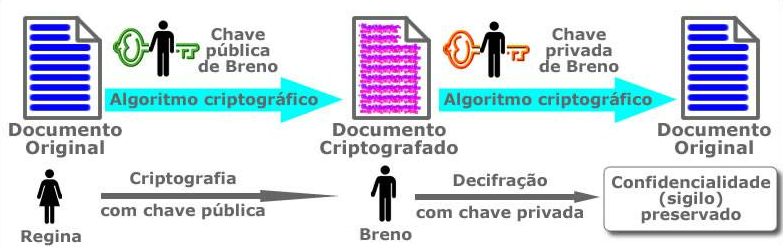
\includegraphics[width=.8\linewidth]{Figuras/Confidencialidade.png}
    \legend{Fonte: }
\end{figure}

A autenticidade garante que quem enviou a mensagem foi o remetente. Quando se tem essa necessidade, deve-se criptografar a mensagem com a chave privada do remetente, enviar a mensagem criptografada para o destinatário, e ele, de posse da chave pública do remetente, poderá decriptografar a mensagem e assim obter a mensagem original.

O fato do destinatário ter conseguido decriptografar a mensagem com a chave pública do remetente comprova que a mensagem é realmente do remetente, mas não garante que o destinatário é o único que poderia decriptografar a mensagem, visto que qualquer pessoa pode possuir a chave pública do remetente, assim como demonstra a Figura 6.

\begin{figure}[H]
    \centering
    \caption{Fluxo da mensagem criptografada quando o foco é autenticidade}
    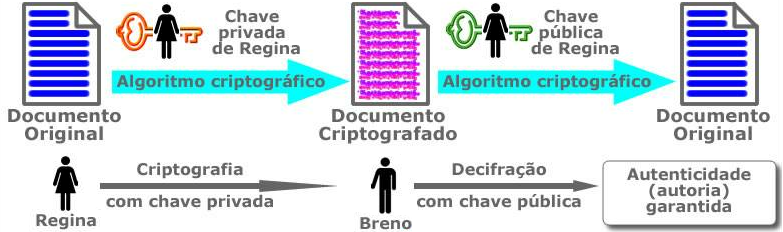
\includegraphics[width=.8\linewidth]{Figuras/Autencidade.png}
    \legend{Fonte: }
\end{figure}

É possível também que se criptografe a mensagem com a chave privada do remetente, criptografar a mensagem já criptografada com a chave pública do destinatário, enviar a mensagem duplamente criptografada para o destinatário, e ele de posse da chave privada, poderá decriptografar a mensagem duplamente criptografada em uma mensagem criptografada e esta por sua vez será decriptografada com a chave pública do remetente e finalmente obter a mensagem original.

A combinação das duas criptografias, a com chave privada do remetente e com a chave publica do receptor, garante tanto que quem vai receber a mensagem é realmente o destinatário correto como garante que o remetente é quem ele diz ser \cite{stallings14}, assim como demonstra a Figura 7.

\begin{figure}[H]
    \centering
    \caption{Fluxo da mensagem criptografada quando o foco é confidencialidade e autenticidade}
    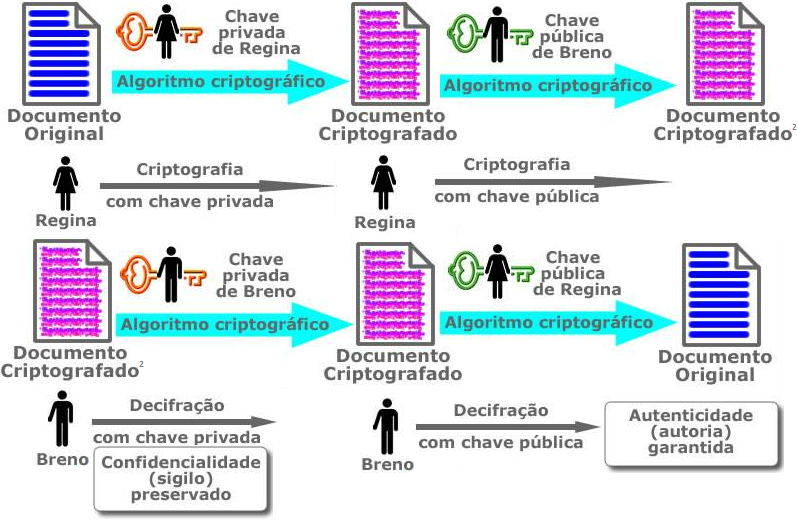
\includegraphics[width=.8\linewidth]{Figuras/ConfidEAuten.png}
    \legend{Fonte: }
\end{figure}

\section{Cifra de blocos}
\label{sec:cifradeblocos}
A cifra de blocos manipula um bloco da mensagem clara como um todo e utiliza este para criar um bloco de mensagem cifrada de mesmo tamanho. É comum a utilização de um bloco com 64 ou 128 bits. Uma cifra de bloco pode ser usada para alcançar o mesmo efeito que uma cifra de fluxo. Cifras de fluxo trata de certo fluxo de dados singularmente, bit a bit ou byte a byte. São implementações clássicas das cifras de fluxo as cifras de \textit{Vigenère} auto chaveada e a cifra de Vernam e a mais utilizada atualmente é o RC4.

A maioria das criptografias simétricas voltadas para ambientes de rede de computadores são implementadas com cifra de blocos e grande parte dos algoritmos de cifra de bloco simétrico usados na atualidade são baseados na cifra de blocos de \textit{Feistel}.

A cifra de bloco trabalha com um bloco de dados da mensagem clara de n bits para produzir um bloco de mensagem cifrada de também de n bits. Se a cifra de bloco se utilizar de um n baixo então a cifra será equivalente a uma cifra de substituição simples. E se n for grande o suficiente e ainda assim for permitida a substituição reversível entre os blocos de mensagem cifrada e não cifrada, então a mensagem clara estaria tão camuflada que a criptoanálise se tornaria inviável.

Uma cifra de substituição reversível qualquer, \textit{Feistel} chamava esse cenário de cifra de bloco ideal, para um grande tamanho de bloco não é viável, do ponto de vista de desempenho e implementação, assim como demonstra a Figura 8.

\begin{figure}[H]
    \centering
    \caption{Cifra de bloco ideal}
    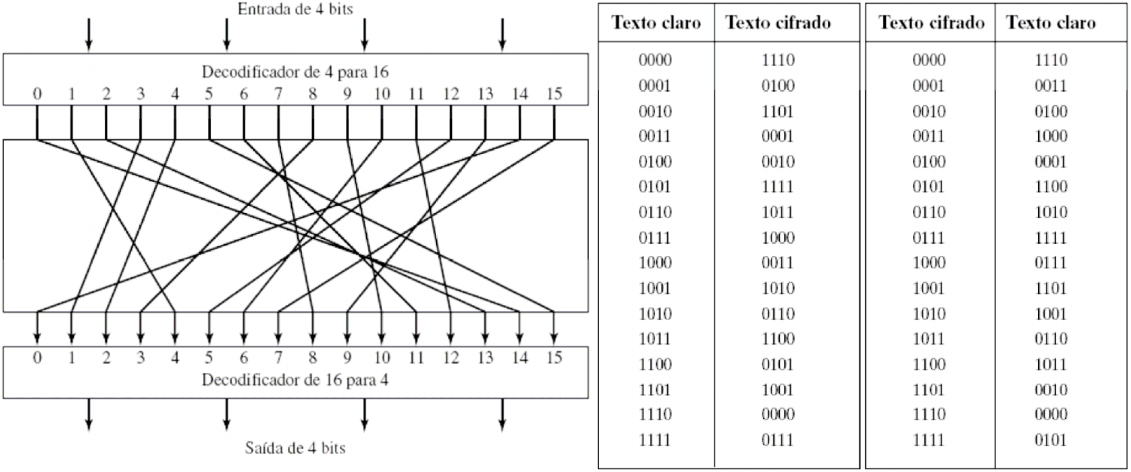
\includegraphics[width=.8\linewidth]{Figuras/CifraDeBloco.png}
    \legend{Fonte: }
\end{figure}

\textit{Feistel} propunha que era possível chegar mais próximo da cifra de bloco ideal. Era só utilizar uma cifra de produto, ou seja, a execução de duas ou mais cifras em sequência, tornando assim o produto final criptograficamente mais forte do que se poderia obter através de qualquer uma das cifras componentes do produto. A estrutura de Feistel consiste em repetidas rodadas do mesmo procedimento. A cada vez que o procedimento se repete é realizada a substituição em metade dos dados da mensagem sendo processados, logo após se permuta as duas metades. A chave sendo utilizada é expandida de modo que uma chave diferente seja utilizada em cada iteração.

Na prática \textit{Fiestel} propôs o uso de uma cifra que alternava entre substituições e permutações, o que na realidade é uma implementação prática do que \textit{Claude Shannon} já havia proposto como, cifra de produto que alterne confusão e difusão \cite{stallings14}.

\section{DES}
\label{sec:des}
Foi estabelecido pela IBM no final da década de 1960 um projeto de pesquisa sobre criptografia de computadores que trazia a sua frente \textit{Horst Feistel}. Com a conclusão do projeto em 1971 foi apresentado como resultado um algoritmo denominado LUCIFER, que foi comercializado ao \textit{Lloyd’s} localizado em Londres para ser utilizado em um sistema de caixa eletrônico que também havia sido desenvolvido pela IBM. LUCIFER é uma cifra de bloco de \textit{Feistel} que operava com blocos de 64 bits e se utilizava de uma palavra com tamanho de 128 bits.

Com o sucesso do LUCIFER a IBM mobilizou um novo projeto, dessa vez com o intuito de tornar o LUCIFER comercializável em grande escala, conseguindo coloca-lo em um único chip. Este projeto, que por sua vez era liderado por \textit{Walter Tuchman} e \textit{Carl Meyer}, contava com a ajuda tanto de consultores externos como orientação técnica da \acrfull{nsa}. O resultado deste novo projeto foi um LUCIFER mais refinado e mais resistente à criptoanálise, mas continha um tamanho de chave de 56 bits, para poder caber em um chip.

A \acrfull{nbs}, em 1973, solicitou propostas de uma cifra para ser padronizada a nível nacional. A IBM enviou o LUCIFER refinado, o que continha 56 bits, e por ser o melhor algoritmo proposto foi, em 1977, adotado como \acrfull{des}.

Com uma chave de 56 bits, existem ao todo 256 possíveis chaves, algo próximo de 7,2 x 1016 chaves. Aparentemente, um número tão grande de possibilidades é algo praticamente impossível de se descobrir se utilizando o método de força bruta. Por exemplo, uma única máquina processando uma criptografia \acrshort{des} por microssegundo levaria mais de mil anos para quebrar a cifra.

Por mais que para as máquinas de hoje, uma criptografia \acrshort{des} a cada microssegundo pareça irreal, pois a velocidade das máquinas de hoje já é bem superior as máquinas da década de 70, para aquela época não era algo tão simples. Mesmo assim, em 1977, \textit{Diffie} e \textit{Hellman} declararam que já existia tecnologia suficiente para se criar uma máquina que concentraria, de forma paralela, um milhão de dispositivos criptográficos, cada um com o poder de processamento da máquina citada no exemplo anterior. Isso reduziria o tempo de quebra da cifra para cerca de dez horas. Infelizmente, tal configuração na época custaria em torno de vinte milhões de dólares.

Finalmente, em 1998, vinte e um anos depois, o \acrshort{des} provou ser inseguro, quando a \acrfull{eff} anunciou que tinha quebrado uma cifra \acrshort{des} utilizando uma máquina “decifradora de DES” montada por menos de 250 mil dólares. Como se isso já não fosse suficiente para tornar o \acrshort{des} um algoritmo criptográfico ultrapassado, ainda existe a constante evolução do hardware, aumentando cada vez mais a velocidade de processamento e consequentemente possibilitando tanto que o método da força bruta seja mais viável, temporalmente falando, como também que sejam criados algoritmos de criptografia que se utilizem melhor desse novo poder de processamento.

Felizmente já existem várias alternativas para o \acrshort{des}, entre elas estão o \acrfull{aes} e o \acrfull{3des} \cite{stallings14}.

\section{3DES}
\label{sec:3des}
A criptografia múltipla é quando um algoritmo de criptografia é utilizado repetidas vezes. Primeiramente, a mensagem clara é criptografada utilizando um algoritmo de criptografia. A mensagem cifrada é então usada como entrada para um algoritmo de criptografia, podendo ser o mesmo utilizado anteriormente ou algum outro algoritmo, e esse processo pode ser repetir por indefinidas vezes.

O \acrfull{3des} é um exemplo de criptografia múltipla. Ele se utiliza do algoritmo \acrshort{des} três vezes, usando duas ou três chaves diferentes.

Em seu estado inicial a criptografia múltipla possui dois estágios, no caso do \acrshort{des} duplo, cada um se utilizando de uma chave diferente uma da outra, a criptografia E de uma mensagem M se utilizando de duas chaves \(K_1\) e \(K_2\) resultando em um texto criptografado C seria assim:

\[C = E(K_2, E(K_1, M))\]

Já a sua decriptografia D seria assim, aplicando as chaves inversamente:

\[M = D(K_1, D(K_2, C))\]

O \acrshort{des} triplo veio como uma alternativa clara para sanar o problema do \acrshort{des} simples, gerado pelo avanço computacional, uma vez que aumenta o custo do ataque da mensagem clara conhecida para 2112 (quando se utiliza de duas chaves) o que está além do possível, pelo menos, atualmente. Mas se utilizar de três estágios com três chaves diferentes exige um tamanho de chave de 168 bits (56 x 3), o que pode ser custoso.

Para diminuir o problema citado, \textit{Tuchman} propôs uma alternativa se utilizando somente de duas chaves:

\[C = E(K_1, D(K_2, E(K_1, M)))\]

A solução acima apresentada se tornou relativamente popular tendo sida adotada para uso nos padrões de gerenciamento de chaves ANS X9.17 e ISO 8732.

Atualmente contra o \acrshort{3des} não existem ataques criptoanalíticos práticos, visto que, o custo de uma pesquisa de chave por força bruta seria de ordem 2112 (quando fossem utilizadas somente duas chaves) o que é equivalente a aproximadamente 5 x 1033. 

Mesmo o \acrshort{3des} com duas chaves sendo de difícil ataque, ainda pode haver uma certa preocupação. Portanto pesquisadores creem que o melhor seria se utilizar do \acrshort{3des} com três chaves. Como já dito anteriormente o \acrshort{3des} com três chaves possui uma chave de tamanho efetivo de 168 bits, o que a torna mais segura em relação com o de duas chaves, e possui a seguinte forma \cite{stallings14}:

\[C = E(K_3, D(K_2, E(K_1, M))\]

\section{S-DES}
\label{sec:sdes}
O \acrfull{sdes}, desenvolvido pelo professor \textit{Edward Schaefer} da \textit{Santa Clara University} \cite{schaefer96}, é uma versão simplificada e voltada ao ensino do algorítimo \acrfull{des} do qual possui as mesmas propriedades e estrutura tendo como únicas divergências o tamanho reduzido dos parâmetros de entrada e o número reduzido de execuções da função \(f_K\). Enquanto o \acrshort{des} recebe como entrada blocos de 64 bits, usa 1 chave de 56 bits de onde se extraem 16 chaves de 48 bits (cada uma será utiliza em uma das 16 aplicações de \(f_K\)) e retorna como saída blocos de 64 bits o \acrshort{sdes} recebe como entrada 1 bloco de 8 bits, usa 1 chave de 10 bits de onde se extraem 2 chaves de 8 bits (cada uma será utilizada em uma das 2 aplicações de \(f_K\)) e retorna como saída 1 bloco de 8 bits. Essas reduções tornam o \acrshort{sdes} o melhor candidato para análise quando o objetivo é aprendizado. \cite{stallings10} \cite{stallings14}

A figura \ref{fig:sdesscheme} apresenta a estrutura geral do \acrshort{sdes}. Nela pode-se observar quais são as etapas que geram as chaves, quais etapas e ordem destas criptografam o \textit{plaintext} e quais etapas e ordem destas descriptografram o \textit{ciphertext}.

\begin{figure}[H]
    \centering
    \caption{Estrutura do \acrshort{sdes}}
    \label{fig:sdesscheme}
    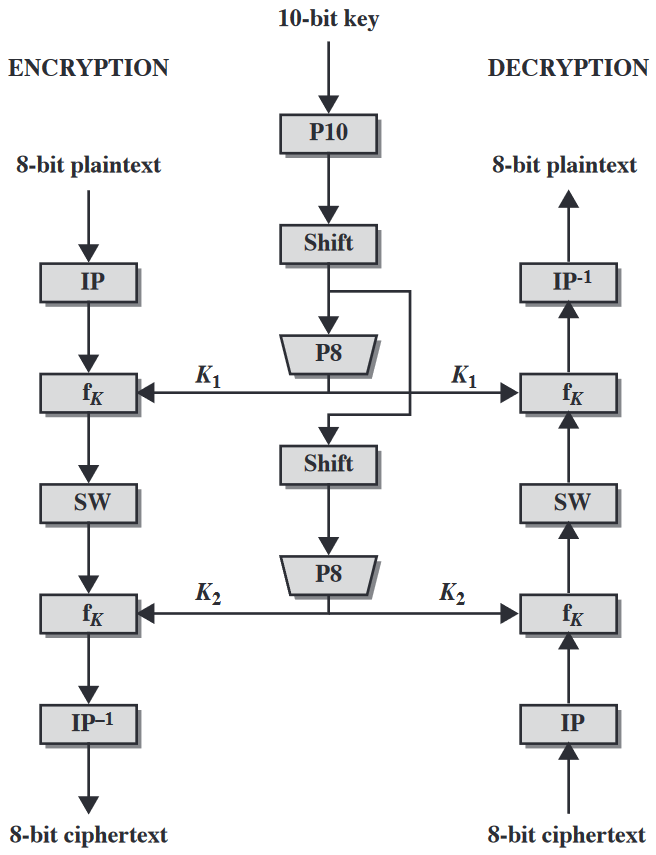
\includegraphics[width=.5\linewidth]{Figuras/SDESScheme.png}
    \legend{Fonte: "Figura G.1 do apêndice G" \cite{stallings10}}
\end{figure}

Pode-se expressar matematicamente o algorítimo de criptografia como uma composição de funções:

\[IP^{-1} \circ f_{K_2} \circ SW \circ f_{K_1} \circ IP\]

Ou de maneira mais direta:

\[ciphertext = IP^{-1}(f_{K_2}(SW(f_{K_1}(IP(plaintext)))))\]

Similarmente pode-se expressar o algorítimo de descriptografia:

\[IP^{-1} \circ f_{K_1} \circ SW \circ f_{K_2} \circ IP\]

Ou também:

\[plaintext = IP^{-1}(f_{K_1}(SW(f_{K_2}(IP(ciphertext)))))\]

\begin{figure}[H]
    \centering
    \caption{Geração das Chaves do \acrshort{sdes}}
    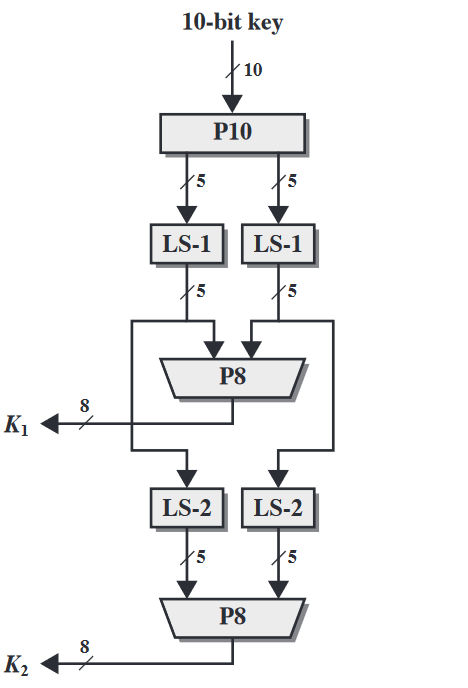
\includegraphics[width=.5\linewidth]{Figuras/SDESKeysGen.png}
    \legend{Fonte: "Figura G.2 do apêndice G" \cite{stallings10}}
\end{figure}

A geração das chaves pode ser expressada através das seguintes:

\[K_1 = P8(Shift_1(P10(key)))\]
\[K_2 = P8(Shift_2(Shift_1(P10(key))))\]

A figura \ref{fig:sdesdetail} demonstra de forma mais detalha o fluxo de execução de criptografia do \acrshort{sdes}. Nesta a função \(f_K\) é detalhada. Esta recebe por sua vez 3 parâmetros: \(L\), \(R\) e \(K\). \(L\) é a metade esquerda dos bits recebidos do passo anterior, \(R\) são os bits restantes, ou seja, a metade direita e \(K\) é a \textit{key} que deve ser utilizada. Sendo assim, temos:

\[f_K(L, R) = (L \oplus F(R, K), R)\]

A função \(F\) por sua vez não é tão facilmente explicita matematicamente mas seu fluxo também pode ser analisado na figura \ref{fig:sdesdetail}. \cite{stallings10}

A descrição detalhada completa do fluxo de execução do \acrshort{sdes} pode ser encontrada no simulador desenvolvido.

\begin{figure}[H]
    \centering
    \caption{Detalhamento da criptografia do \acrshort{sdes}}
    \label{fig:sdesdetail}
    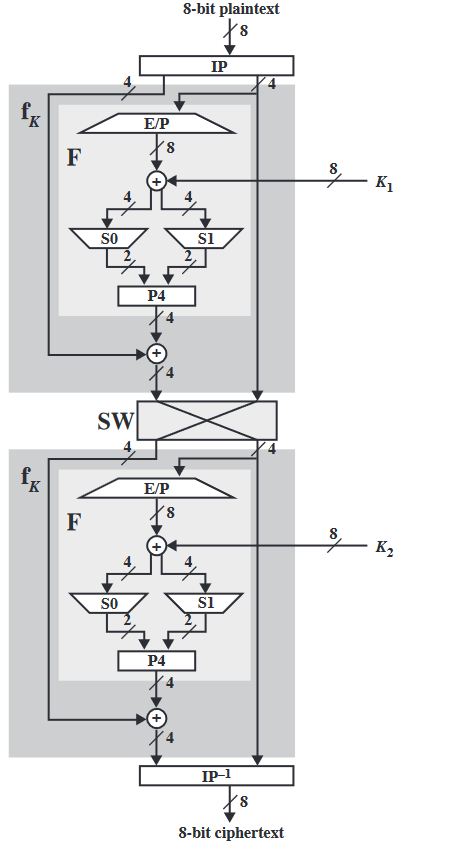
\includegraphics[width=.5\linewidth]{Figuras/SDESEncrypDetail.png}
    \legend{Fonte: "Figura G.3 do apêndice G" \cite{stallings10}}
\end{figure}

\chapter{O simulador}
\label{char:ferrdesenvolvida}
Esse capítulo descreve o \textbf{CryptoEdu - simulador de algoritmos de criptografia com finalidade educacional} criado no decorrer da escrita desse trabalho de conclusão de curso.

O simulador permite a execução completa e passo a passo de todas as etapas envolvidas tanto na criptografia quando na descriptografia utilizando o algoritimo \acrfull{sdes}, escolhido por ser um algoritmo mais recomendado para ensino, como explicado na seção \ref{sec:sdes}.

O público alvo da ferramenta é o corpo docente e discente de cursos de TI. Mas também, pode ser utilizada por todos que desejam aprender como a criptografia de cifra de blocos funcionada, refinar e/ou lapidar os conhecimentos já adquiridos ou até somente desmistificar esse conteúdo complexo chamado criptografia.

\section{Informações técnicas}

O simulador foi desenvolvido na linguagem \textit{Javascript} utilizando \textit{React.js} e \textit{Typescript}. O ambiente de desenvolvimento utilizado foi o \textit{Visual Studio Code}. O código fonte do simulador é \textit{open source} e está disponibilizado no \textit{GitHub} no endereço \textit{https://github.com/TanielianVB/CryptoEdu/}.

No \textit{GitHub} é possível: Gerenciar problemas encontrados e melhorias sugeridas através de \textit{Issues}.; Integrar melhorias implementados por terceiros através de \textit{Pull Requests}.; A publicação de qualquer nova versão está automatizada através da ferramenta \textit{Netlify} (\textit{https://www.netlify.com/}) e reagindo à qualquer nova versão submetida ao repositório. Esses \textit{deploys} podem ser visualizados em \textit{https://app.netlify.com/sites/cryptoedu/deploys/}.; E até, caso necessário, criar uma nova versão do simulador de propriedade de terceiros através do \textit{Fork}.

O simulador está disponibilizado ao usuário através da internet no endereço \textit{https://cryptoedu.netlify.app/}. O simulador pode ser visualizado em \textit{browsers}, inclusive em dispositivos móveis. No entanto a melhor experiência é obtida quando se utiliza uma resolução maior. Normalmente só obtida se utilizando \textit{desktops}.

\section{Estrutura da interface}
Nessa seção são descritos os elementos contidos na interface de maneira estrutural.

\begin{figure}[H]
    \centering
    \caption{Estrutura da interface}
    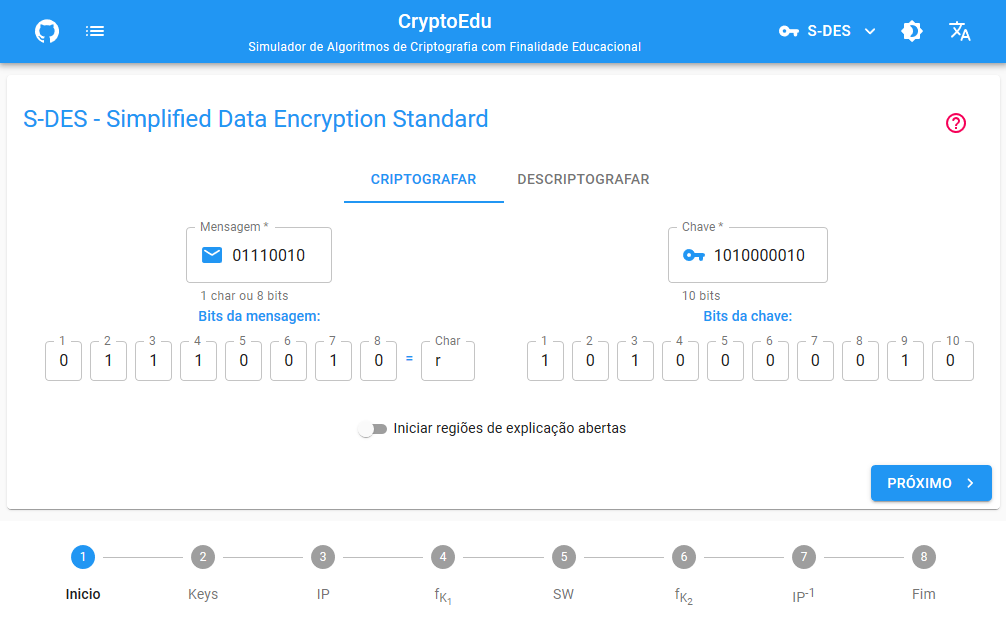
\includegraphics[width=1\linewidth]{UI/UIEstrutura.png}
\end{figure}

\subsection{Cabeçalho}

\begin{figure}[H]
    \centering
    \caption{Cabeçalho}
    
\includegraphics[width=1\linewidth]{UI/UIHeader.png}
\end{figure}

A região do cabeçalho possui:
\begin{itemize}
    \item Link do repositório onde está localizado tanto o código fonte do simulador como um pdf do TCC: \textit{https://github.com/TanielianVB/CryptoEdu}
    \item Link do questionário de \textit{feedback} de utilização do simulador.
    \item O nome do simulador: \textbf{CryptoEdu - Simulador de Algoritmos de Criptografia com Finalidade Educacional}.
    \item \textit{Combo Box} de escolha do algoritmo que está em execução.
    \item Botão para alternar entre o tema \textbf{claro} e \textbf{escuro}.
    \item Botão para alterar o idioma no qual o simulador está sendo exibido.
\end{itemize}

\subsection{Conteúdo}

\begin{figure}[H]
    \centering
    \caption{Conteúdo}
    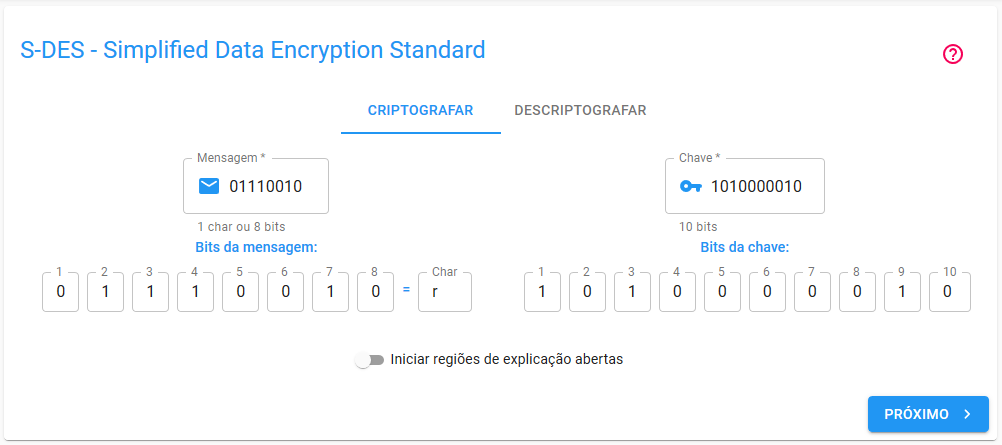
\includegraphics[width=1\linewidth]{UI/UIMain.png}
\end{figure}

A região principal da página será onde cada passo da execução do algoritmo selecionado irá ocorrer. Em cada passo serão listados as etapas executadas em cada passo.

Inicialmente irá conter uma interface discorrendo sobre o algoritmo selecionado e posteriormente cada passo que estará sendo executado. É possível navegar por esses passos através dos botões de navegação (Próximo e Anterior) exibidos na parte inferior da região de cada passo. No último passo o botão Próximo é substituído pelo botão Reiniciar para facilitar o início de uma nova execução.

\subsection{Rodapé}

\begin{figure}[H]
    \centering
    \caption{Rodapé}
    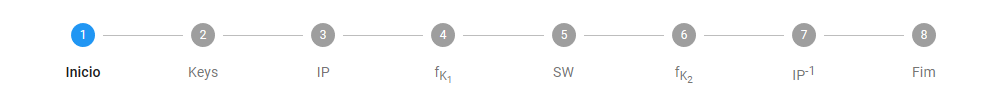
\includegraphics[width=1\linewidth]{UI/UIFooter.png}
\end{figure}

A região do rodapé contém:
\begin{itemize}
    \item Todos os passos necessários para a execução do algoritmo em execução. Ao se passar o mouse sobre eles é exibida uma \textit{tooltip} com um nome mais explicativo do passo.
    \item Quais passos já foram completados.
    \item Qual passo o usuário se encontra no momento.
    \item Quais passos ainda faltam ser completados para finalizar a execução do algoritmo.
\end{itemize}
É possível também, a qualquer momento, navegar para qualquer passo diretamente. Basta-se clicar sobre este.

\subsection{\textit{Mobile}}

\begin{figure}[H]
    \centering
    \caption{Visualização em um \textit{browser} de dispositivo móvel}
    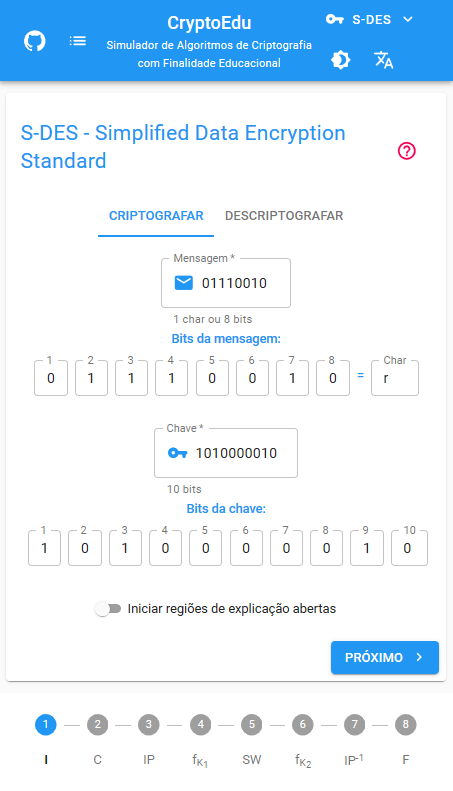
\includegraphics[width=0.5\linewidth]{UI/UIMobile.png}
\end{figure}

Embora não seja o ideal, o simulador se comporta bem em dispositivos móveis melhorando ainda mais a sua acessibilidade.

\section{Interface do conteúdo}
Descrição da interface apresentada em cada um dos passos da execução do algoritmo.

Cada passo possui no mínimo uma etapa e cada etapa possui uma região de explicação onde a etapa é descrita de maneira que possibilite o usuário compreender como a etapa é executada, como essa deve ser compreendida, como esta difere de outras etapas similares e qual a definição matemática desta etapa, caso haja.

A explicação pode ser acessada através do clique do botão interrogação à direita do cabeçalho que contém o título da referida etapa. Esse clique irá expandir a região que contém a explicação da etapa. É possível também que todas as regiões de explicação já iniciem abertas. Basta habilitar a opção \textbf{Iniciar regiões de explicação abertas} ao iniciar a execução da criptografia ou descriptografia.

\subsection{Tela inicial - entrada de dados}

\begin{figure}[H]
    \centering
    \caption{Tela inicial - entrada de dados}
    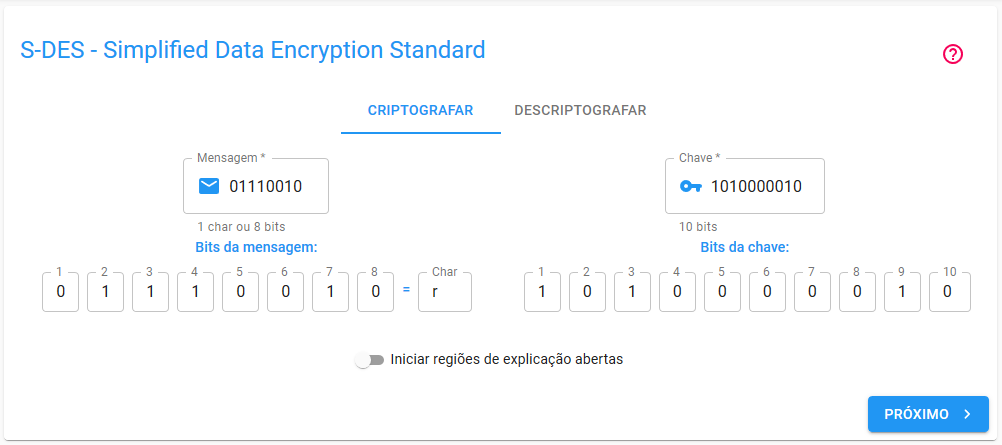
\includegraphics[width=1\linewidth]{UI/UIMain.png}
\end{figure}

A interface inicial faz uma breve descrição do algoritmo selecionado na \textit{Combo Box} de escolha de algoritmo buscando situar o usuário no contexto selecionado para execução. No momento só será disponibilizado um algoritmo: \acrfull{sdes}.

O usuário pode então escolher se ele deseja o fluxo de execução \textbf{criptografar} ou \textbf{descriptografar} e assim então informar valores customizados para os campos \textbf{Mensagem} (\textbf{Mensagem cifrada} caso o fluxo escolhido tenha sido o \textbf{descriptografar}) e \textbf{Chave}.

Os algoritmos recebem como entrada bits. Por conta disso, são exibidos os bits contidos nos campos e que serão utilizados para a execução do fluxo escolhido. Tanto para facilitar o preenchimento do campo \textbf{Mensagem} como para melhorar a compreensão do usuário sobre o valor contido no campo, é possível informar no campo uma letra, visto que essa pode, e é, facilmente convertida para 8 bits. Isso ajuda não somente no preenchimento do campo durante a execução do fluxo \textbf{criptografar} mas também na validação do resultado obtido da execução do fluxo \textbf{descriptografar} visto quê é possível, mais facilmente, comparar as mensagens (tanto a de entrada do fluxo \textbf{criptografar} quando a de saída do fluxo \textbf{descriptografar}) se estas forem letras. Exemplo: A letra \textbf{'T'} gera a sequência de bits: \textbf{01010100}.

Nessa tela também é possível habilitar a opção \textbf{Iniciar regiões de explicação abertas} que fará com que, durante a navegação pelos passos da execução do algoritmo todas as regiões de explicação já se iniciem abertas. Caso o usuário não queria mais visualizar a explicação para alguma etapa. Ele pode esconder a explicação clicando no botão à direita do título da etapa.

\subsection{Passo Chaves - Geração das chaves}

Nesse passo estão concentradas todas as etapas necessárias para a geração das chaves \(K_1\) e \(K_2\). A etapas contidas nesse passo estavam inicialmente divididas em 3 passos. Mas por ter gerado dúvida sobre como essas etapas se relacionavam tanto entre elas como com os outros passos da execução do algoritmo estas etapas estão em um mesmo passo.

\subsubsection{Etapa P10 - Permutação de 10 bits}

\begin{figure}[H]
    \centering
    \caption{Etapa P10 - Permutação de 10 bits}
    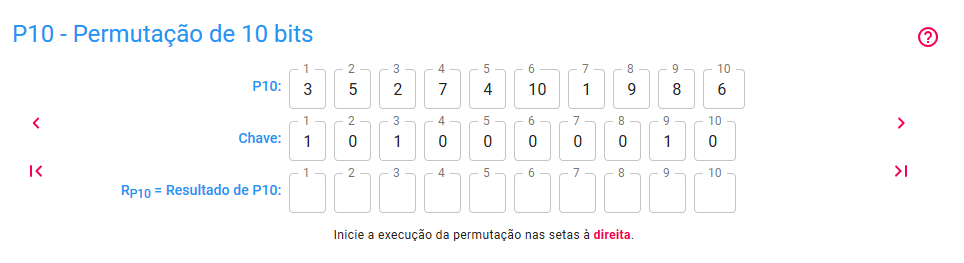
\includegraphics[width=1\linewidth]{UI/UIP10.png}
\end{figure}

A interface da etapa P10 contextualiza o objetivo pelo qual essa etapa existe, explica a definição de uma função de permutação, apresenta a função de permutação P10 (incluindo função matemática) e explica como esta deve ser interpretada. Após tal contextualização se exibe um componente capaz de executar passo a passo a função de permutação P10. O parâmetro de entrada da permutação P10 é a Chave recebida da tela de entrada de dados. O resultado dessa execução será o parâmetro de entrada para a próxima etapa, LS-1.

\subsubsection{Etapa LS-1 - \textit{Circular Left Shift} de 1 posição}

\begin{figure}[H]
    \centering
    \caption{Etapa LS-1 - \textit{Circular Left Shift} de 1 posição}
    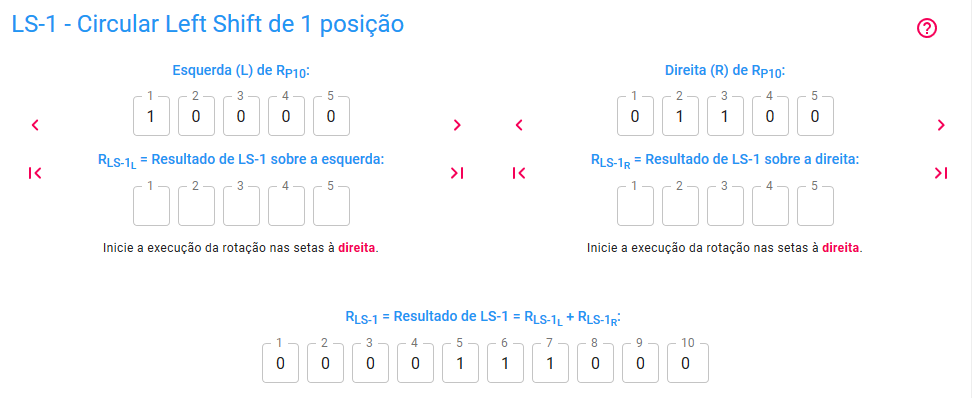
\includegraphics[width=1\linewidth]{UI/UILS1.png}
\end{figure}

A interface da etapa LS-1 contextualiza o objetivo pelo qual essa etapa existe e explica como esta etapa deve ocorrer, incluindo a divisão na metade do valor obtido na etapa anterior (P10) e o que é o processo de rotação. Após tal contextualização se exibe dois componentes capazes de executar passo a passo a rotação circular para a esquerda de 1 posição. Cada um destes componentes irá rotacionar uma das metades. O resultado desta etapa é então a junção das metades após suas rotações individuais.

\subsubsection{Etapa P8 - Permutação de 8 bits sobre o resultado de LS-1}

\begin{figure}[H]
    \centering
    \caption{Passo P8 - Permutação de 8 bits sobre o resultado de LS-1}
    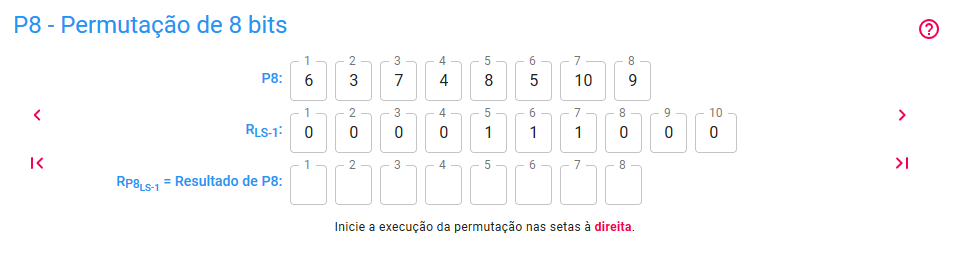
\includegraphics[width=1\linewidth]{UI/UIP81.png}
\end{figure}

A interface da etapa P8 contextualiza o objetivo pelo qual essa etapa existe, explica a definição de uma função de permutação, apresenta a função de permutação P8 (incluindo função matemática) e explica como esta deve ser interpretada. Após tal contextualização se exibe um componente capaz de executar passo a passo a função de permutação P8. O parâmetro de entrada da permutação P8 é o resultado obtido na etapa anterior, LS-1.

\subsubsection{Resultado Chave \(K_1\)}

\begin{figure}[H]
    \centering
    \caption{Chave \(K_1\) - Geração da primeira chave \(K_1\)}
    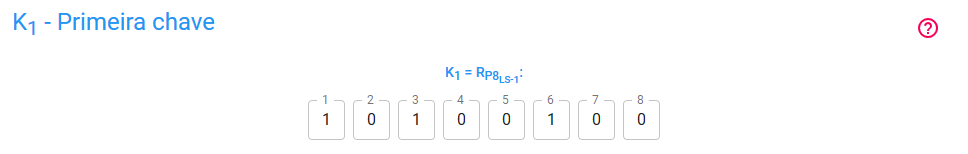
\includegraphics[width=1\linewidth]{UI/UIK1.png}
\end{figure}

O resultado da aplicação da função de permutação P8 sobre o resultado da etapa LS-1 será a primeira chave K1. Esta será utilizada em uma etapa futura durante a criptografia ou descriptografia da mensagem.

\subsubsection{Etapa LS-2 - \textit{Circular Left Shift} de 2 posições}

\begin{figure}[H]
    \centering
    \caption{Etapa LS-2 - \textit{Circular Left Shift} de 2 posições}
    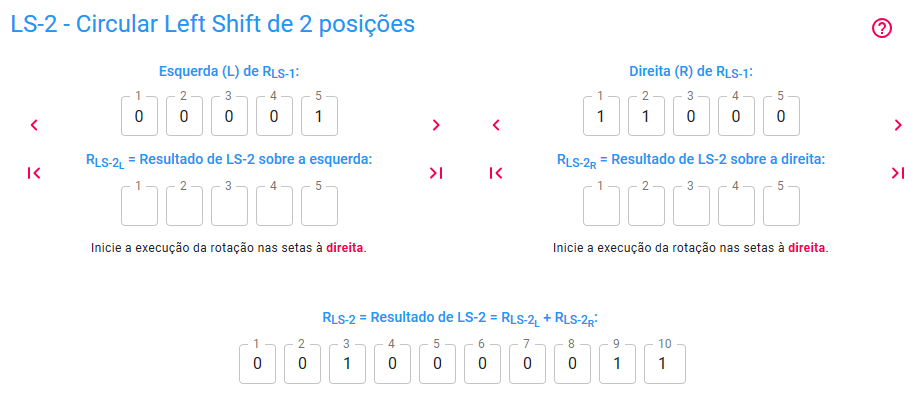
\includegraphics[width=1\linewidth]{UI/UILS2.png}
\end{figure}

A interface da etapa LS-2 contextualiza o objetivo pelo qual essa etapa existe e explica como esta etapa deve ocorrer, incluindo a divisão na metade do valor obtido na etapa LS-1 e o que é o processo de rotação. Após tal contextualização se exibe dois componentes capazes de executar passo a passo a rotação circular para a esquerda de 2 posições. Cada um destes componentes irá rotacionar uma das metades. O resultado desta etapa é então a junção das metades após suas rotações individuais.

\subsubsection{Etapa P8 - Permutação de 8 bits sobre o resultado de LS-2}

\begin{figure}[H]
    \centering
    \caption{Passo P8 - Permutação de 8 bits sobre o resultado de LS-2}
    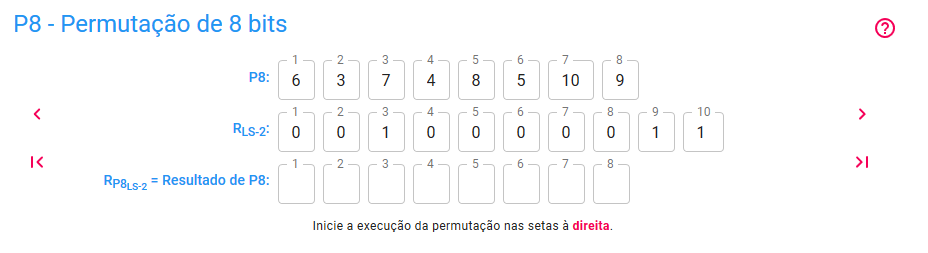
\includegraphics[width=1\linewidth]{UI/UIP82.png}
\end{figure}

A interface da etapa P8 contextualiza o objetivo pelo qual essa etapa existe, explica a definição de uma função de permutação, apresenta a função de permutação P8 (incluindo função matemática) e explica como esta deve ser interpretada. Após tal contextualização se exibe um componente capaz de executar passo a passo a função de permutação P8. O parâmetro de entrada da permutação P8 é o resultado obtido na etapa anterior, LS-2.

\subsubsection{Resultado Chave \(K_2\)}

\begin{figure}[H]
    \centering
    \caption{Chave \(K_2\) - Geração da segunda chave \(K_2\)}
    
\includegraphics[width=1\linewidth]{UI/UIK2.png}
\end{figure}

O resultado da aplicação da função de permutação P8 sobre o resultado da etapa LS-2 será a segunda chave K2. Esta será utilizada em uma etapa futura durante a criptografia ou descriptografia da mensagem.

\subsection{Passo IP - Permutação Inicial}

\begin{figure}[H]
    \centering
    \caption{Passo IP (\textit{Initial Permutation}) - Permutação Inicial}
    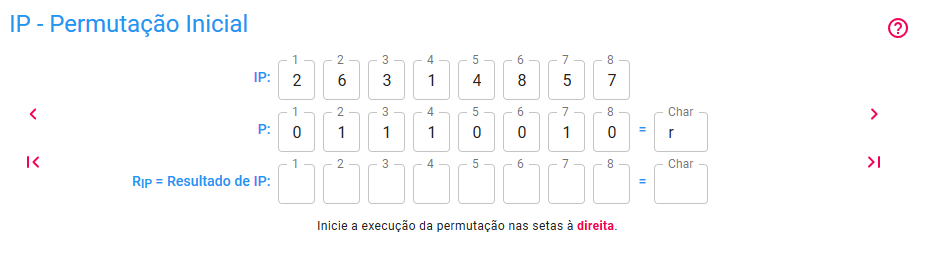
\includegraphics[width=1\linewidth]{UI/UIIP.png}
\end{figure}

A interface da etapa IP contextualiza o objetivo pelo qual essa etapa existe, explica a definição de uma função de permutação, apresenta a função de permutação IP (incluindo função matemática) e explica como esta deve ser interpretada. Após tal contextualização se exibe um componente capaz de executar passo a passo a função de permutação IP. O parâmetro de entrada da permutação IP é a Mensagem (\textit{Plaintext} P) recebida da tela de entrada de dados.

\begin{figure}[H]
    \centering
    \caption{L (esquerda) \& R (direita)}
    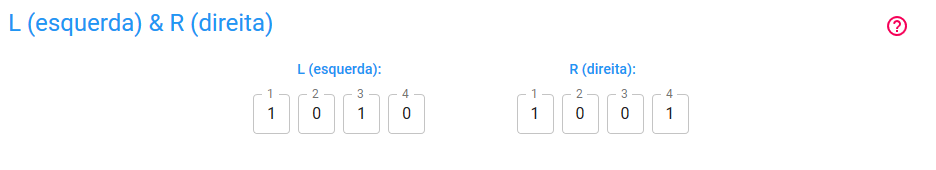
\includegraphics[width=1\linewidth]{UI/UILR.png}
\end{figure}

O resultado desse passo é a divisão do resultado obtido da permutação IP em duas metades, L (\textit{left}) e R (\textit{right}), que serão enfim passados por parâmetro para a execução da função \(f_K\).

\subsection{Passo \(f_K\) - Função que usa uma chave}

\begin{figure}[H]
    \centering
    \caption{Passo \(f_K\) - Função que usa uma chave}
    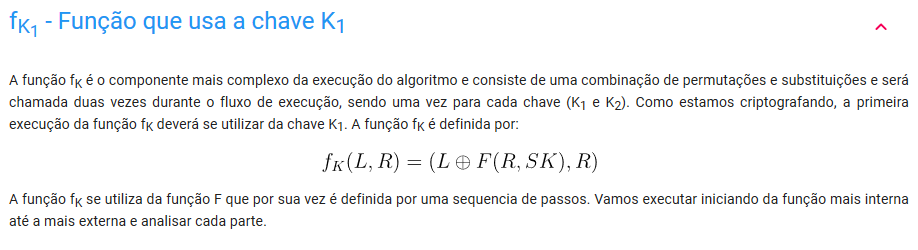
\includegraphics[width=1\linewidth]{UI/UIFK1.png}
\end{figure}

Esse passo é o único passo que se repete durante a execução da criptografia ou descriptografia. Essa função recebe 2 parâmetros de entrada. Um é uma sequência de 8 bits divididos entre L \& R (4 bits na esquerda L e 4 bits na direita R) e o segundo parâmetro é a chave. Caso a execução escolhida seja a criptografia, a primeira vez que essa função é executada a chave utilizada será a \(K_1\) e na segunda vez será a \(K_2\). Caso a execução escolhida seja a descriptografia, a ordem de utilização das chaves será inversa. A interface explica a tais peculiaridades e apresenta a função matemática desta.

Nesse passo estão concentradas todas as etapas da execução da função \(f_K\). A etapas contidas nesse passo estavam inicialmente divididas em 2 passos. Um indo até o primeiro XOR e outro indo até o segundo XOR. Mas por esse passo se repetir optou-se por deixar todas as etapas em um único passo.

\subsubsection{Etapa E/P - Permutação de Expansão}

\begin{figure}[H]
    \centering
    \caption{Etapa E/P - Permutação de Expansão}
    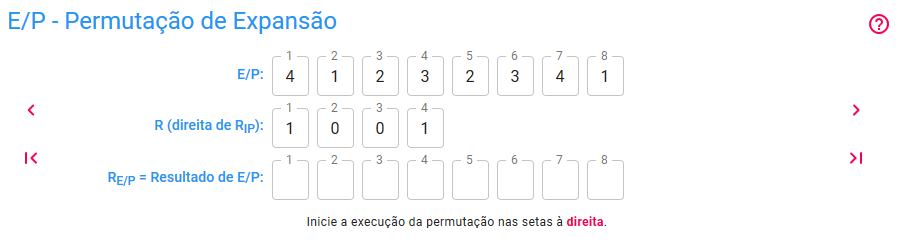
\includegraphics[width=1\linewidth]{UI/UIEP.png}
\end{figure}

A interface da etapa E/P contextualiza o objetivo pelo qual essa etapa existe, explica a definição de uma função de permutação, apresenta a função de permutação E/P (incluindo função matemática) e explica como esta deve ser interpretada. Após tal contextualização se exibe um componente capaz de executar passo a passo a função de permutação E/P. O parâmetro de entrada da permutação E/P é o parâmetro de entrada R da função \(f_K\) (4 bits do lado direito dos 8 bits recebidos de entrada).

\subsubsection{Etapa XOR - OU exclusivo com \(K_1\)}

\begin{figure}[H]
    \centering
    \caption{Etapa XOR - OU exclusivo com \(K_1\)}
    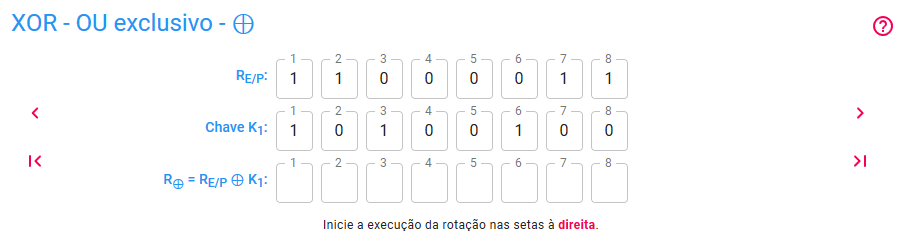
\includegraphics[width=1\linewidth]{UI/UIXORK1.png}
\end{figure}

A interface da primeira etapa XOR descreve o que ocorre nessa etapa e exibe um componente capaz de executar bit a bit a operação XOR (OU exclusivo) para obtenção do resultado dessa etapa. Os parâmetros de entrada dessa etapa são: 1. O resultado da permutação de expansão E/P e 2. Ou a chave \(K_1\) ou a chave \(K_2\). Caso a execução escolhida seja a criptografia, a primeira vez que essa etapa é executada a chave utilizada será a \(K_1\) e na segunda vez será a \(K_2\). Caso a execução escolhida seja a descriptografia, a ordem de utilização das chaves será inversa. A interface reflete essas particularidades em cada fluxo de execução.

\subsubsection{Etapa S0 \& S1 - Substituições S0 e S1}

\begin{figure}[H]
    \centering
    \caption{Etapa S0 \& S1 - Substituições S0 e S1}
    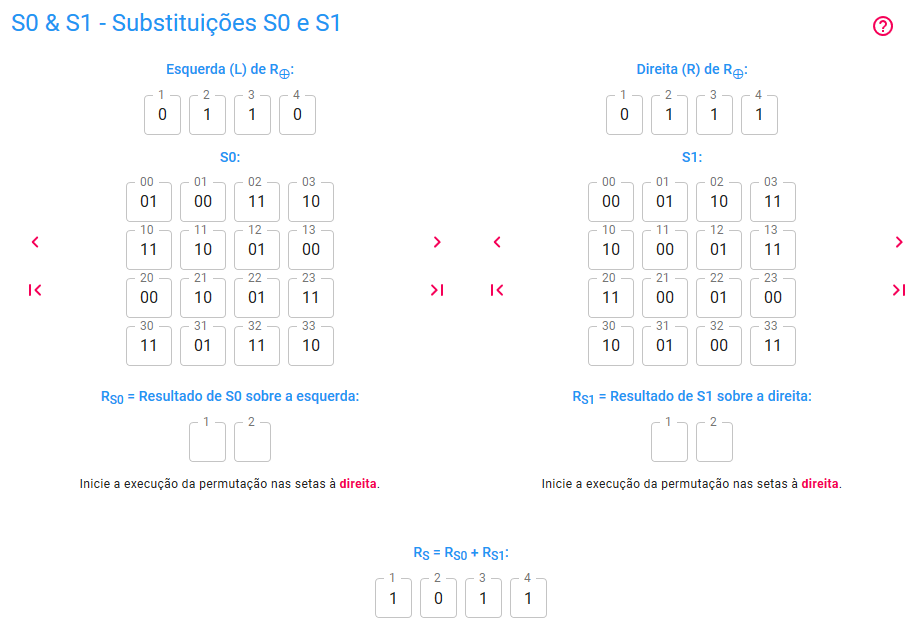
\includegraphics[width=1\linewidth]{UI/UIS0S1.png}
\end{figure}

A interface da etapa das substituições S0 e S1 contextualiza o objetivo pelo qual essa etapa existe, explica a definição de um substituição, apresenta a obtenção dos parâmetros de entrada para cada substituição e explica como uma substituição deve ser interpretada. Após tal contextualização se exibe, para cada substituição, um componente capaz de executar passo a passo a substituição. Os parâmetros de entrada das substituições S0 e S1 são, respectivamente, as metades esquerda e direita do resultado obtido na etapa anterior (XOR com \(K_1\)). O resultado desta etapa é então a junção das metades após suas substituições individuais.

\subsubsection{Etapa P4 - Permutação de 4 bits}

\begin{figure}[H]
    \centering
    \caption{Etapa P4 - Permutação de 4 bits}
    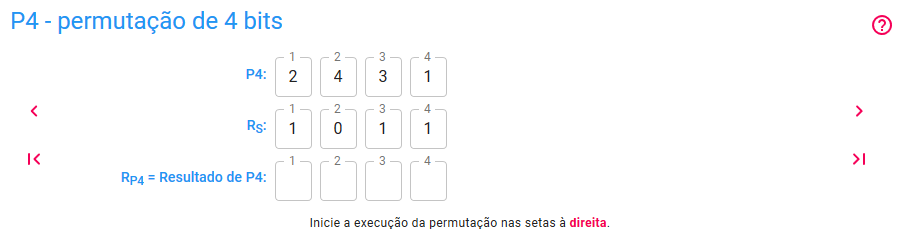
\includegraphics[width=1\linewidth]{UI/UIP4.png}
\end{figure}

A interface da etapa P4 contextualiza o objetivo pelo qual essa etapa existe, explica a definição de uma função de permutação, apresenta a função de permutação P4 (incluindo função matemática) e explica como esta deve ser interpretada. Após tal contextualização se exibe um componente capaz de executar passo a passo a função de permutação P4. O parâmetro de entrada da permutação P4 é o resultado obtido na etapa anterior (Substituições S0 e S1). O resultado dessa execução será o parâmetro de entrada para a próxima etapa, XOR com L.

\subsubsection{Etapa XOR - OU exclusivo com L}

\begin{figure}[H]
    \centering
    \caption{Etapa XOR - OU exclusivo com L}
    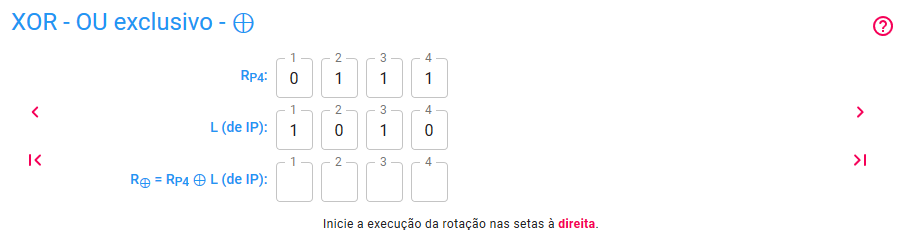
\includegraphics[width=1\linewidth]{UI/UIXORL.png}
\end{figure}

A interface da segunda etapa XOR descreve o que ocorre nessa etapa e exibe um componente capaz de executar bit a abit a operação XOR (OU exclusivo) para obtenção do resultado dessa etapa. Os parâmetros de entrada dessa etapa são: 1. O resultado da permutação P4 e 2. L (metade esquerda do parâmetro de entrada de \(f_K\)). Na primeira vez que \(f_K\) é executada L será a esquerda do resultado da permutação inicial (IP) e na segunda vez L será a esquerda do resulta da Troca (SW).

\subsubsection{Resultado de \(f_K\)}

\begin{figure}[H]
    \centering
    \caption{Resultado de \(f_K\)}
    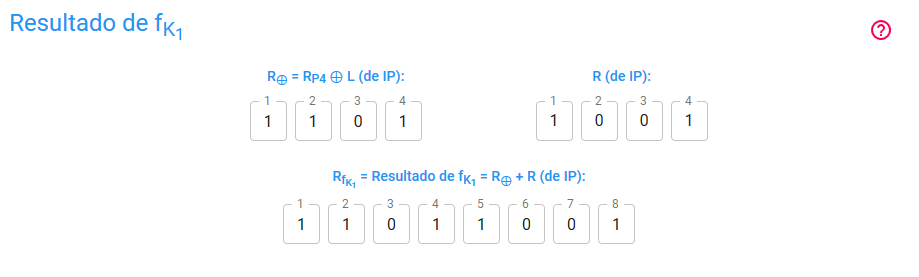
\includegraphics[width=1\linewidth]{UI/UIRFK1.png}
\end{figure}

A interface do resultado de \(f_K\) exibe as metades que compõem o resultado da função e a junção destes. A metade esquerda desse resultado sempre será o resultado da etapa anterior, XOR. A metade direita será a metade direita do parâmetro de entrada da função \(f_K\). Que na primeira vez é a metade direita do resultado da permutação inicial (IP) e na segunda vez é a matade direita da Troca (SW).

\subsection{Passo SW - Troca}

\begin{figure}[H]
    \centering
    \caption{Passo SW - Troca}
    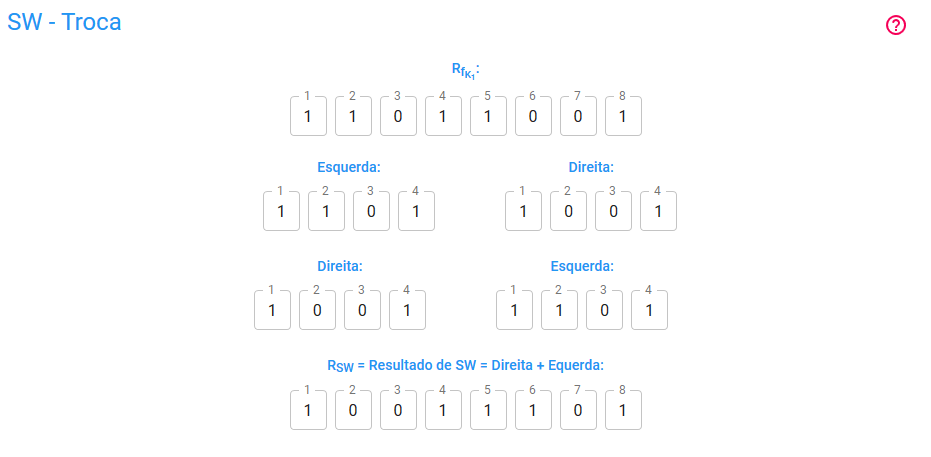
\includegraphics[width=1\linewidth]{UI/UISW.png}
\end{figure}

A interface do passo Troca (SW) explica a definição da troca, apresenta a função de troca (incluindo função matemática) e explica como esta deve ser interpretada. Este é o passo intermediário entre as execuções das funções \(f_K\). Ela recebe por parâmetro o resultado da primeira execução da função \(f_K\) e o resultado deste passo é o parâmetro de entrada para a segunda execução da função \(f_K\) juntamente com a chave que não foi utilizada pela primeira execução.

\subsection{Passo \(f_K\) - Função que usa a outra chave}

A segunda execução da função \(f_K\) é sequencialmente idêntica à primeira logo as interfaces de cada etapa são similares. As únicas diferenças são:
\begin{itemize}
    \item O parâmetro de entrada é o resultado do passo Troca (SW) e não o resultado do passo Permutação inicial (IP) como ocorre na primeira execução da função.
    \item A chave utilizada é a chave que não foi utilizada na primeira execução da função \(f_K\). Na criptografia a primeira execução da função \(f_K\) utiliza a chave \(K_1\) e a segunda execução a chave \(K_2\). Já na descriptografia o inverso é verdade. A interface identifica o fluxo que está sendo executado e reflete essas diferenças tanto nas \textit{labels} quanto nas explicações das etapas.
\end{itemize}

\subsection{Passo \(IP^{-1}\) - Permutação Inicial Inversa}

\begin{figure}[H]
    \centering
    \caption{Passo \(IP^{-1}\) - Permutação Inicial Inversa}
    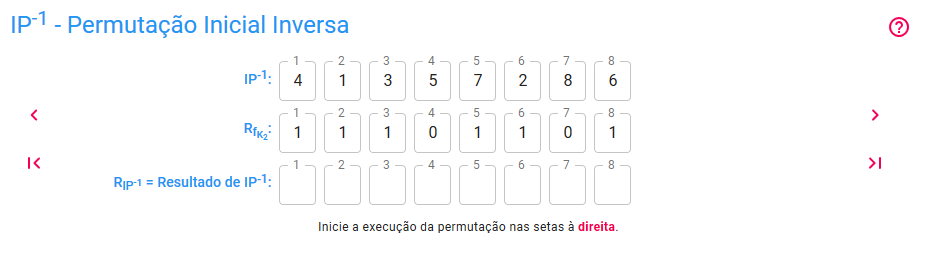
\includegraphics[width=1\linewidth]{UI/UIIP-1.png}
\end{figure}

A interface da etapa \(IP^{-1}\) contextualiza o objetivo pelo qual essa etapa existe, explica a definição de uma função de permutação, apresenta a função de permutação \(IP^{-1}\) (incluindo função matemática) e explica como esta deve ser interpretada. Após tal contextualização se exibe um componente capaz de executar passo a passo a função de permutação \(IP^{-1}\). O parâmetro de entrada da permutação \(IP^{-1}\) é o resultado obtido no passo anterior (\(f_K\)).

\subsection{Tela final - Resultado}

\begin{figure}[H]
    \centering
    \caption{Resultado}
    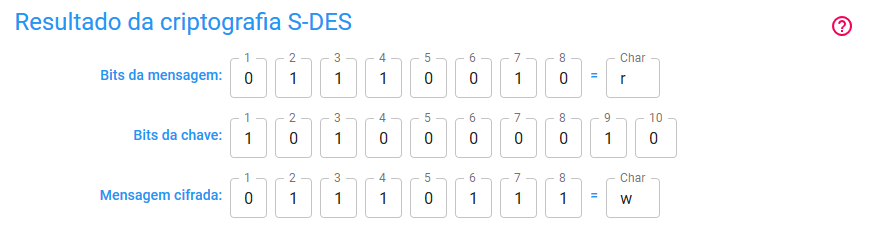
\includegraphics[width=1\linewidth]{UI/UIResult.png}
\end{figure}

A interface do último passo exibe os dois parâmetros de entrada da execução, a Mensagem e a Chave, e o resultado da execução da criptografia ou descriptografia.

\begin{figure}[H]
    \centering
    \caption{\textit{Feedback request}}
    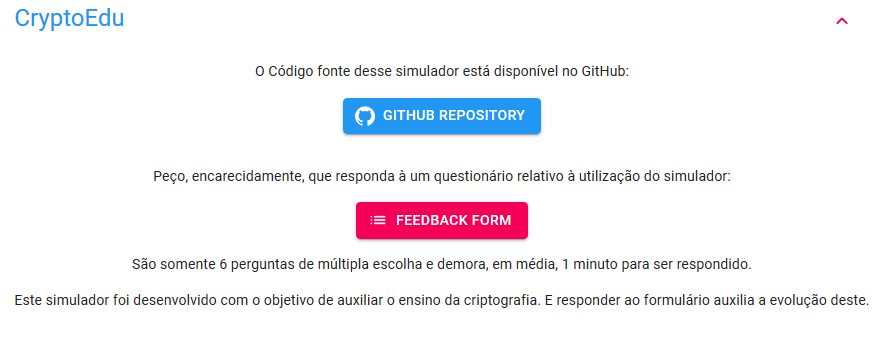
\includegraphics[width=1\linewidth]{UI/UIFeedback.png}
\end{figure}

O último ponto na interface é uma solicitação do preenchimento do questionário de utilização do simulador. É exibido também um link para o repositório \textit{GitHub} onde se encontra o simulador. No \textit{GitHub} também é possível baixar a última versão publicada deste \acrshort{tcc}.

\section{Limites da solução}
A ferramenta foi desenvolvida prevendo uma fácil extensão das suas atuais funcionalidades. Mas, visto que o escopo do projeto pode, facilmente, se exceder além do limite possível de execução de um trabalho de conclusão de curso, alguns limites foram impostos para viabilizar o desenvolvimento da ferramenta em tempo hábil. São eles:
\begin{itemize}
    \item Somente 1 algoritmo será disponibilizado. Sendo este, o \acrfull{sdes}.
    \item Só estará disponibilizado no tema \textbf{claro}.
    \item Só estará disponibilizado em \textbf{Português-BR}.
    \item A interface terá foco para dispositivos \textit{desktop}.
\end{itemize}

\section{Comparação com outros simuladores criptográficos}
Os simuladores foram comparados em alguns pontos: \textbf{Idioma}; \textbf{Algoritmos}, quais algoritmos o simulador é capaz de simular; \textbf{Educativo}, se o simulador é voltado ao ensino ou não; \textbf{I/O}, nível de detalhamento das entradas e saídas, em que, \textbf{algoritmo} exibe somente as entradas e saídas do algoritmo, \textbf{passo} exibe também as entradas e saídas de cada passo do algoritmo e \textbf{etapa} exibe também as entradas e saídas de cada etapa dentro de cada passo; \textbf{\textit{Open Source}}, se o simulador possui código aberto e permite ou não que colaboradores extendam suas funcionalidades; \textbf{Plataforma}; e \textbf{Responsivo}, que indica o nível de responsividade da interface do simulador.

Comparando o simulador desenvolvido com os outros simuladores criptográficos encontrados, levando em consideração os pontos já explícitos, temos:

\begin{table}[h!]
\centering
    \addtolength{\leftskip} {-3cm} % increase (absolute) value if needed
    \addtolength{\rightskip}{-2cm}
\resizebox{1.2\textwidth}{!}{%
\begin{tabular}{ c | c c c c c c }
 \xrowht{20pt} & \textbf{CyberChef} & \textbf{CrypTool} & \textbf{S-DES Sim. App} & \textbf{S-DES Sim. \textit{online}} & \textbf{S-DES Sim. Win} & \textbf{CryptoEdu} \\
 \hline
 \xrowht{20pt} \textbf{Idioma} & Inglês & Inglês & Inglês & Koreano & Inglês & \cellcolor{green!70!yellow!40} Português \\
 \xrowht{20pt} \textbf{Algoritmos} & Vários & Vários & \cellcolor{green!70!yellow!40} S-DES & \cellcolor{green!70!yellow!40} S-DES & \cellcolor{green!70!yellow!40} S-DES & \cellcolor{green!70!yellow!40} S-DES \\
 \xrowht{20pt} \textbf{Educativo} & Não & \cellcolor{green!70!yellow!40} Sim & \cellcolor{green!70!yellow!40} Sim & \cellcolor{green!70!yellow!40} Sim & \cellcolor{green!70!yellow!40} Sim & \cellcolor{green!70!yellow!40} Sim \\
 \xrowht{20pt} \textbf{I/O} & algoritmo & algoritmo & passo & passo & passo & \cellcolor{green!70!yellow!40} etapa \\
 \xrowht{20pt} \textbf{\textit{Open Source}} & \cellcolor{green!70!yellow!40} Sim & Não & Não & \cellcolor{green!70!yellow!40} Sim & Não & \cellcolor{green!70!yellow!40} Sim \\
 \xrowht{20pt} \textbf{Plataforma} & \cellcolor{green!70!yellow!40} \textit{online} & SO's & Android & \cellcolor{green!70!yellow!40} \textit{online} & Windows & \cellcolor{green!70!yellow!40} \textit{online} \\
 \xrowht{20pt} \textbf{Responsivo} & \textit{desktop} & \textit{desktop} & \cellcolor{green!70!yellow!40} \textit{mobile} & \textit{desktop} & \textit{desktop} & \cellcolor{green!70!yellow!40} \textit{desktop} e \textit{mobile} \\
\end{tabular}}
\end{table}

Foram marcados de verde, na tabela, os pontos dos simuladores que se sobressaem quando analisados em um contexto de acessibilidade e ensino-aprendizagem.

%\begin{itemize}
    %\item É mais acessível. Somente 2 dos outros simuladores estão \textit{online}, nenhum deles é utilizável em \textit{mobile}, destes somente 1 é voltado para o ensino e este está em Koreano. 
    %\item Possui detalhamento da execução do algoritmo. Embora alguns outros simuladores sejam voltados ao ensino, nenhum deles explica o processo que ocorre dentro das etapas do algoritmo muito menos permite uma execução passo a passo dos processos contidos nessas etapas.
%\end{itemize}

\chapter{Pesquisa de reação}
\label{char:pesquisa}
Com o intuito de mensurar de forma real o alcance dos objetivos propostos neste trabalho, foi proposta uma pesquisa de reação sobre a utilização do simulador. Essa pesquisa possui 6 perguntas, 1 relativa ao usuário, 3 relativas à absorção de conhecimento oriundas da utilização do simulador e 2 relativas à melhorias que podem ser feitas no simulador.

O questionário de \textit{feedback} de utilização do simulador foi disponibilizado, através da utilização do \textit{Google Forms} através do link \textit{https://forms.gle/f1DAgWvTyM2uJyLt9}.

\begin{figure}[H]
    \centering
    \caption{Inicio do questionário}
    \label{fig:inicioquestionario}
    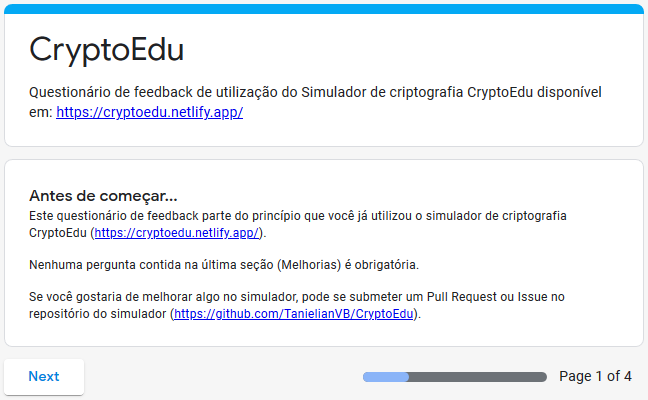
\includegraphics[width=0.75\linewidth]{Questionario/QI.png}
    \legend{Fonte: do autor}
\end{figure}

Antes de propor as questões para o usuário, é exibida essa tela de apresentação do questionário (figura \ref{fig:inicioquestionario}).

\section{Perguntas}
O questionário é composto de 6 perguntas, sendo 4 obrigatórias e 2 opcionais, que serão descritas à seguir.

Um fator que foi levado em consideração ao desenvolver o  questionário é a dificuldade de adquirir respostas dos usuários. Por esse motivo e para facilitar a análise dos resultados optou-se por utilizar somente de perguntas de múltipla escolha.

\subsection{Enquadramento do usuário}

\begin{figure}[H]
    \centering
    \caption{Enquadramento do usuário}
    \label{fig:enquadramentousuario}
    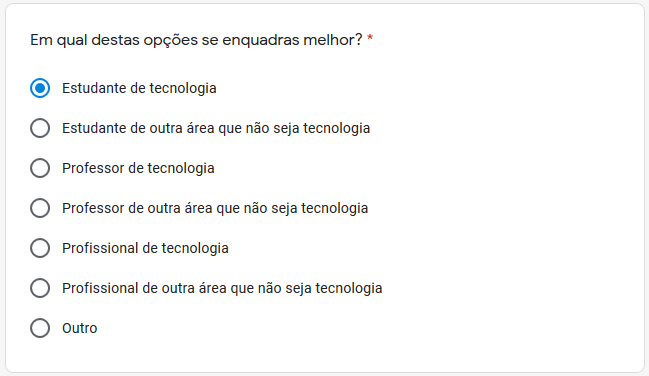
\includegraphics[width=0.75\linewidth]{Questionario/Q1.png}
    \legend{Fonte: do autor}
\end{figure}

Esta pergunta (figura \ref{fig:enquadramentousuario}) tem como objetivo ter uma \textit{baseline} do tipo de usuário que está respondendo o questionário e, dessa forma, ser capaz de obter uma curva de crescimento por 'perfil'.

\subsection{Conhecimento antes e depois da utilização do simulador}
As próximas 2 perguntas objetivam mensurar se houve evolução do nível de conhecimento dos usuários sobre os processos de criptografia presentes na simulação do algoritmo S-DES. O escopo das perguntas envolve os processos (permutação, rotação, substituição, xor e troca) presentes no algoritmo, em vez das etapas (P10, LS-1, P8, LS-2, IP, etc...), pois munido do conhecimento dos processos todas as etapas podem ser reproduzidas.

\begin{figure}[H]
    \centering
    \caption{Conhecimento antes da utilização do simulador}
    \label{fig:conhecimentoantes}
    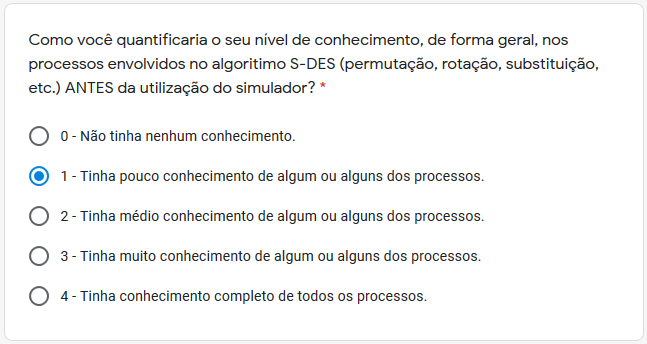
\includegraphics[width=0.75\linewidth]{Questionario/Q2.png}
    \legend{Fonte: do autor}
\end{figure}

Para mensurar se houve evolução do nível de conhecimento, é questionado primeiramente como o usuário quantificaria o nível de conhecimento, de maneira geral, que ele possui nos processos presentes no algoritmo antes da utilização do simulador (figura \ref{fig:conhecimentoantes}). Buscando obter o ponto de partida do nível de conhecimento.

\begin{figure}[H]
    \centering
    \caption{Conhecimento depois da utilização do simulador}
    \label{fig:conhecimentodepois}
    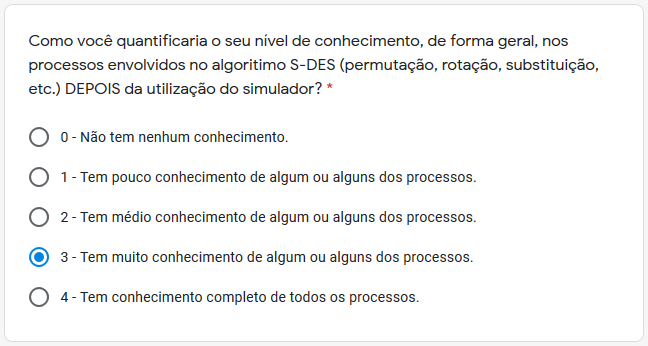
\includegraphics[width=0.75\linewidth]{Questionario/Q3.png}
    \legend{Fonte: do autor}
\end{figure}

A próxima pergunta indaga esse mesmo nível de conhecimento após a utilização do simulador (figura \ref{fig:conhecimentodepois}). Buscando obter o ponto de chegada do nível de conhecimento.

\subsection{Efetividade do aprendizado}

\begin{figure}[H]
    \centering
    \caption{Efetividade do aprendizado}
    \label{fig:efetividadeaprendizado}
    \includegraphics[width=0.75\linewidth]{Questionario/Q4.png}
    \legend{Fonte: do autor}
\end{figure}

Esta pergunta (figura \ref{fig:efetividadeaprendizado}) tem como objetivo mensurar, de maneira absoluta, se existiu ganho de conhecimento por parte do usuário.

\subsection{Melhorias no simulador}
Com as próximas 2 perguntas tem-se como objetivo ser capaz de identificar quais etapas explícitas no simulador precisam ser melhoradas. O escopo das perguntas envolve as etapas (P10, LS-1, P8, LS-2, IP, etc...) presentes no algoritmo, em vez dos processos (permutação, rotação, substituição, xor e troca), pois cada descrição e execução é singular àquela determinada etapa.

\begin{figure}[H]
    \centering
    \caption{Melhorias nas descrições das etapas}
    \label{fig:melhoriadescricoes}
    \includegraphics[width=0.7\linewidth]{Questionario/Q5.png}
    \legend{Fonte: do autor}
\end{figure}

A primeira pergunta (figura \ref{fig:melhoriadescricoes}) desta seção destina-se à identificar quais etapas da execução do algoritmo possuem explicações que podem ser melhoradas, ou seja, não foram suficientes para compreensão completa da etapa pelo usuário.

\begin{figure}[H]
    \centering
    \caption{Melhorias nas execuções das etapas}
    \label{fig:melhoriaexecucoes}
    \includegraphics[width=0.7\linewidth]{Questionario/Q6.png}
    \legend{Fonte: do autor}
\end{figure}

A segunda pergunta (figura \ref{fig:melhoriaexecucoes}) desta seção destina-se a identificar quais etapas da execução do algoritmo possuem execuções (passo a passo) que podem ser melhoradas, ou seja, não foram suficientes para compreensão completa do passo a passo da etapa pelo usuário.

\section{Resultados da pesquisa}

Esta seção descreve os resultados da pesquisa realizada. A pesquisa contou com a participação de alunos e professores da \acrshort{fbuni} e da \acrshort{unifor}, como também de profissionais das seguintes empresas: Unimake, RCN e Fortes Tecnologia.

\subsection{Enquadramento do usuário}

\begin{figure}[H]
    \centering
    \caption{Enquadramento do usuário}
    \label{fig:enquadramentousuarioresp}
    \includegraphics[width=.65\linewidth]{Questionario/CQ1.png}
    \legend{Fonte: do autor}
\end{figure}

Foram obtidas 65 respostas. Sendo 86,2\% da área tecnológica em que 43,1\% são estudantes, 30,8\% profissionais e 12,3\% professores (figura \ref{fig:enquadramentousuarioresp}). Embora esse montante não seja o suficiente para um estudo do ponto de vista estatístico, é suficiente para mensurar a efetividade da ferramenta desenvolvida.

\subsection{Conhecimento antes e depois da utilização do simulador}

\begin{figure}[H]
    \centering
    \caption{Conhecimento antes vs. depois da utilização do simulador por enquadramento}
    \label{fig:conhecimentoantesdepoisresp}
    \includegraphics[width=.9\linewidth]{Questionario/CQ2Q3.png}
    \legend{Fonte: do autor}
\end{figure}

Analisando o nível de conhecimento antes e depois para cada enquadramento (figura \ref{fig:conhecimentoantesdepoisresp}), temos:

\begin{itemize}
    \item Estudantes de tecnologia apresentaram um aumento médio de 1,68 pontos. A média de conhecimento antes era entre \textbf{nenhum} ou \textbf{pouco} e após a utilização do simulador passou a ser \textbf{médio} ou superior.
    \item Profissionais de tecnologia apresentaram um aumento médio de 1,05 pontos. A média de conhecimento antes era \textbf{pouco} e, após a utilização do simulador, passou a ser \textbf{médio} ou superior.
    \item Professores de tecnologia apresentaram um aumento médio de 1,88 pontos. A média de conhecimento antes era entre \textbf{pouco} ou \textbf{médio} e após a utilização do simulador passou a ser \textbf{muito} ou superior.
\end{itemize}

Infelizmente, não foram obtidos dados suficientes dos outros enquadramentos que tornasse viável extrair qualquer tipo de conclusão sobre estes.

\subsection{Efetividade do aprendizado}

\begin{figure}[H]
    \centering
    \caption{Efetividade do aprendizado}
    \label{fig:efetividadeaprendizadoresp}
    \includegraphics[width=.65\linewidth]{Questionario/CQ4.png}
    \legend{Fonte: do autor}
\end{figure}

95,4\% dos entrevistados consideram que o seu nível de conhecimento sobre os processos e etapas apresentados no simulador melhorou após a utilização do simulador (figura \ref{fig:efetividadeaprendizadoresp}). Um ponto interessante é que mesmo alguns entrevistados que se avaliaram no mesmo nível de conhecimento antes e depois da utilização do simulador ainda assim alegaram ter aprendido com ele.

\subsection{Melhorias no simulador}

\begin{figure}[H]
    \centering
    \caption{Melhorias no simulador}
    \label{fig:melhoriasresp}
    \includegraphics[width=.9\linewidth]{Questionario/CQ5Q6.png}
    \legend{Fonte: do autor}
\end{figure}

Somente 21,53\% dos entrevistados apontaram que algumas etapas poderiam ser melhoradas (figura \ref{fig:melhoriasresp}). Dentre os pontos de melhoria apontado, as descrições das permutações e substituição foram os mais indicados como pontos que precisam de melhoria.

\chapter{Conclusões e Trabalhos futuros}
\label{char:conclusoesetrabfuturos}
Esta pesquisa abordou a temática de \acrfull{oa} da Informática na Educação.

Inicialmente, levantou-se os desafios do processo de ensino-aprendizagem da criptografia no meio acadêmico, ressaltando a necessidade desse conhecimento para o formando, independentemente de seguir carreira acadêmica ou de TI. A complexidade dos algoritmos aliada ao tempo normalmente disponível ao ensino desses são elementos que dificultam o processo de ensino-aprendizagem, mas isso pode ser mitigado com ferramentas voltadas ao ensino criptográfico.

Vale ressaltar o aumento contínuo do uso dos \acrshort{oas} no meio acadêmico em razão das vantagens provenientes de seu uso no processo ensino-aprendizagem, como: o auxílio de ensino presencial e principalmente à distância (\acrshort{ead}), sua acessibilidade, e grande interação entre o usuário e o \acrshort{oa}. Como exemplo de \acrshort{oa}, temos o jogo \textit{Minecraft: Education Edition} que já foi aplicado no ensino de Biologia, Ecologia, Física, Química, Geologia, Geografia e até Cibersegurança.

O simulador resultado da pesquisa realizada trás avanços e contribuições para a área da Informática Educacional, dos quais destacam-se: é em português; é o primeiro a apresentar explicação e execução passo a passo de todas as etapas, de cada passo, envolvidas tanto no processo de criptografia como no processo de descriptografia; e é mais acessível pois pode ser visualizado tanto em \textit{desktop} como em \textit{mobile}.

O simulador foi disponibilizado para uma comunidade de alunos e professores a fim de avaliar, por meio de uma pesquisa, a sua efetividade no processo de ensino-aprendizagem da técnica de criptografia por cifra de blocos. Esta efetividade se fez comprovada quando, após a utilização do simulador, \textbf{95,4\%} dos entrevistados consideraram que melhoraram o seu nível de conhecimento sobre os processos e etapas nele apresentados. Além disso, alunos de tecnologia passaram a ter nível de conhecimento \textbf{médio} sobre esses mesmos processos e etapas quando o seu nível de conhecimento original era \textbf{nenhum} ou \textbf{pouco}.

Como possíveis trabalhos futuros, sugere-se: aplicar ao simulador melhorias nos aspectos escolhidos pelos entrevistados como pontos que podem ser melhorados, tornando, assim, o simulador ainda mais eficiente no ensino-aprendizagem; adicionar outros algoritmos ao simulador, dessa forma, aumentando seu nicho de aplicabilidade.


\phantompart % necessário

% ----------------------------------------------------------
% ELEMENTOS PÓS-TEXTUAIS
% ----------------------------------------------------------
\postextual

% ----------------------------------------------------------
% Referências bibliográficas
% ----------------------------------------------------------
%\bibliographystyle{abbrv}
\bibliography{0c_referencias}

%---------------------------------------------------------------------
% INDICE REMISSIVO
%---------------------------------------------------------------------
\phantompart
\printindex

\end{document}
